%%
%% Copyright 2021 OXFORD UNIVERSITY PRESS
%%
%% This file is part of the 'ima-authoring-template Bundle'.
%% ---------------------------------------------
%%
%% It may be distributed under the conditions of the LaTeX Project Public
%% License, either version 1.2 of this license or (at your option) any
%% later version.  The latest version of this license is in
%%    http://www.latex-project.org/lppl.txt
%% and version 1.2 or later is part of all distributions of LaTeX
%% version 1999/12/01 or later.
%%
%% The list of all files belonging to the 'ima-authoring-template Bundle' is
%% given in the file `manifest.txt'.
%%
%% Template article for OXFORD UNIVERSITY PRESS's document class `ima-authoring-template'
%% with bibliographic references
%%

\documentclass[webpdf, namedate]{ima-authoring-template}
%\documentclass[namedate,webpdf]{ima-authoring-template}

%\usepackage{showframe}

\usepackage[utf8]{inputenc}
\usepackage[T1]{fontenc}
\usepackage{url}
\usepackage{tikz}
\usepackage{geometry}
\usepackage{caption}
\usepackage{xurl}
\usepackage{microtype}

 \usetikzlibrary{arrows.meta, shapes.geometric, shapes.multipart, fit, positioning, backgrounds, shadows}

% \geometry{margin=1in}
\setlength{\emergencystretch}{10em}
\overfullrule=0pt

% line numbers
%\usepackage[mathlines, switch]{lineno}
%\usepackage[right]{lineno}

\theoremstyle{thmstyletwo}%
\newtheorem{theorem}{Theorem}%  meant for continuous numbers
%%\newtheorem{theorem}{Theorem}[section]% meant for sectionwise numbers
%% optional argument [theorem] produces theorem numbering sequence instead of independent numbers for Proposition
\newtheorem{proposition}[theorem]{Proposition}%
%%\newtheorem{proposition}{Proposition}% to get separate numbers for theorem and proposition etc.

\newtheorem{example}{Example}%
\newtheorem{remark}{Remark}%

\newtheorem{definition}{Definition}

\numberwithin{equation}{section}

\begin{document}

\DOI{DOI HERE}
\copyrightyear{2026}
\vol{00}
\pubyear{2026}
\access{Advance Access Publication Date: Day Month Year}
\appnotes{Paper}
% \copyrightstatement{Published by Oxford University Press on behalf of the Institute of Mathematics and its Applications. All rights reserved.}
\firstpage{1}

%\subtitle{Subject Section}

\title[Automated Clinical Audio-to-FHIR Pipeline]{Designing an Automated Pipeline for Mapping Unstructured Clinical Audio to HL7 FHIR-Compliant Data Structures}

\author{Dauren Baimurza*
\address{\orgdiv{Computer Science}, \orgname{SDU University}, \orgaddress{\street{Street}, \postcode{Postcode}, \state{Almaty}, \country{Kazakhstan}}}}
\authormark{Dauren Baimurza}

\corresp[*]{Corresponding author: \href{email:email-id.com}{email-id.com}}

\received{Date}{0}{Year}
\revised{Date}{0}{Year}
\accepted{Date}{0}{Year}

%\editor{Associate Editor: Name}


\abstract{Abstracts must be able to stand alone and so cannot contain citations to
the paper's references, equations, etc. An abstract must consist of a single
paragraph and be concise. Because of online formatting, abstracts must appear
as plain as possible.}
\keywords{Automatic Speech Recognition; Speaker Diarization; Clinical Audio Processing; Large Language Models; Clinical Information Extraction; HL7 FHIR; Healthcare Interoperability.}

% \boxedtext{
% \begin{itemize}
% \item Key boxed text here.
% \item Key boxed text here.
% \item Key boxed text here.
% \end{itemize}}

\maketitle
\section{Introduction}

\subsection{Background and Problem Statement}

The digitization of healthcare systems over the past two decades has led to exponential growth in the volume of clinical data generated across care settings. However, despite widespread adoption of Electronic Health Record (EHR) systems, a substantial proportion of clinically valuable information remains locked in unstructured formats — including physician dictations, bedside observations, referral notes, and patient-provider conversations. Studies have consistently demonstrated that unstructured data, when appropriately processed, contributes meaningfully to clinical tasks such as phenotyping and quality measurement, yet it remains largely inaccessible to automated systems in its raw form \cite{hong2020nlp2fhir}.

The coexistence of structured and unstructured data in healthcare presents both a challenge and an opportunity. Structured data — stored in coded fields and controlled vocabularies — enables systematic querying and analysis, while unstructured data often captures the richness, nuance, and context of clinical encounters that structured forms cannot convey \cite{hong2017integrating, brens2025semantic}. Empirical studies have quantified this complementarity: across 172 clinical phenotypes derived from MIMIC-III, textual features outperform structured measurements alone for 84\% of phenotypes, with their combination yielding statistically significant improvements for phenotypes where context recorded in clinical notes is not reflected in tabular measurements \cite{moldwin2021phenotyping}. Bridging this divide has long been recognized as a fundamental informatics challenge: extracting meaningful, computable representations from free-text and audio-based clinical content requires not only language understanding but also domain-specific knowledge and semantic reasoning \cite{builtjes2025leveraging}.

Beyond text, clinical audio represents perhaps the most underutilized modality in health informatics. Encounters between patients and clinicians — whether in outpatient consultations, emergency settings, or telehealth platforms — generate continuous streams of spoken dialogue that contain diagnostically and clinically relevant content. The conversion of this audio into structured, actionable data remains overwhelmingly manual, relying on transcriptionists, clinical coders, or clinicians themselves to document encounters post hoc. This process is time-consuming, prone to inconsistency, and contributes significantly to the administrative burden placed on healthcare providers \cite{saadat2025enhancing, klusty2024clinical}.

\subsection{The Role of HL7 FHIR in Healthcare Interoperability}

HL7 Fast Healthcare Interoperability Resources (FHIR) has emerged as the leading international standard for the representation and exchange of healthcare information. By defining a modular, resource-based data model — encompassing clinical entities such as \texttt{Patient}, \texttt{Encounter}, \texttt{Observation}, \texttt{Condition}, and \texttt{MedicationRequest} — FHIR enables semantic interoperability across disparate health information systems \cite{hl7fhir2022r4b}. Recent work applying large language models to FHIR transformation has demonstrated a broad range of applications, including clinical decision support, patient data exchange, population health management, and regulatory reporting, while also highlighting persistent implementation challenges such as terminology binding, resource profiling complexity, and inconsistent adoption across jurisdictions \cite{li2024fhirgpt}.

The adoption of FHIR as a mandated or preferred interoperability standard by major healthcare regulators — including the U.S.\ Office of the National Coordinator for Health IT — has accelerated its uptake globally. Despite this progress, the vast majority of FHIR-compliant data structures are populated from existing structured EHR fields. The generation of FHIR resources from unstructured sources, particularly spoken clinical audio, remains an understudied and largely unsolved problem. Automating this pathway would not only reduce transcription burden but also enable real-time or near-real-time population of clinical records, supporting downstream analytics, care coordination, and research reuse.

\subsection{Automatic Speech Recognition in Healthcare}

Automatic Speech Recognition (ASR) technologies have undergone a paradigm shift in capability and accessibility, driven by deep learning architectures and large-scale pretraining. Radford et al.\ introduced Whisper, a general-purpose ASR model trained on 680,000 hours of multilingual, weakly supervised audio data, demonstrating near-human transcription accuracy and robust zero-shot generalization across diverse acoustic domains \cite{radford2023whisper}. The accessibility of such pretrained models makes them compelling candidates for integration into clinical audio processing pipelines, eliminating the need to train ASR systems from scratch.

The application of ASR in healthcare settings carries distinctive challenges that differentiate clinical speech from general-domain audio. Medical terminology is highly specialized, acoustically dense with domain-specific vocabulary (e.g., drug names, anatomical terms, diagnostic codes), and often produced under challenging recording conditions — background noise, overlapping speakers, and informal conversational register. Independent evaluation of both general-purpose and specialized ASR models on real patient-clinician conversations has confirmed that, even under controlled recording conditions, clinical dialogue yields word error rates of 8.8–10.5\% alongside variable speaker diarization accuracy \cite{tran2022asr}. The PriMock57 dataset — comprising 57 recorded mock primary care consultations with manual transcriptions — provides a key benchmark for evaluating ASR systems under realistic clinical dialogue conditions \cite{papadopoulos2022primock57}.

Recent work has explored the use of Large Language Models (LLMs) as post-processing layers to improve ASR output quality in medical transcription. Adedeji et al.\ demonstrated that applying LLMs — particularly through Chain-of-Thought (CoT) prompting — to refine ASR-generated transcripts of primary care consultations improved both general and medical-concept word error rates, while also enhancing speaker diarization accuracy and semantic coherence \cite{adedeji2024sound}. These findings collectively suggest that a hybrid pipeline — combining a pretrained ASR system with LLM-based post-processing — represents a practical and effective approach to medical transcription without requiring custom model development.

\subsection{From Transcription to Structured Clinical Data}

Transcription alone is insufficient for clinical informatics applications. To be computationally actionable, spoken clinical content must be transformed into structured representations grounded in standard terminologies and data models. This requires NLP pipelines capable of named entity recognition, relation extraction, negation detection, and normalization against controlled vocabularies such as SNOMED CT, LOINC, and RxNorm. The extraction of clinical information from unstructured data — including clinical notes and transcribed encounters — has been demonstrated as feasible using open-source LLMs in zero-shot settings, though accuracy varies substantially by entity type and documentation style \cite{builtjes2025leveraging}.

Mapping extracted clinical concepts to FHIR resources introduces an additional layer of complexity. Each FHIR resource type carries specific structural requirements, terminology bindings, and cardinality constraints that must be satisfied to produce conformant output. The challenge of designing a pipeline that traverses the full pathway from raw audio to validated FHIR resource instances — integrating ASR, NLP, terminology normalization, and resource generation — has not been comprehensively addressed in the literature. Existing approaches tend to address individual stages in isolation, leaving the end-to-end integration as an open engineering and research problem \cite{hong2020nlp2fhir, riquelme2025llm}.

\subsection{Research Objectives and Scope}

This study presents the design and evaluation of an automated pipeline for mapping unstructured clinical audio to HL7 FHIR Release 4B-compliant data structures \cite{hl7fhir2022r4b}. Rather than developing novel ASR or NLP models from scratch, the proposed system integrates and orchestrates existing pretrained components — including Whisper \cite{radford2023whisper} for transcription and LLM-based processing for clinical entity identification \cite{adedeji2024sound} — within a unified, modular architecture. The pipeline is developed and evaluated using the PriMock57 dataset of primary care mock consultations \cite{papadopoulos2022primock57}. By utilizing a dataset consisting of mock consultations with professional actors, this research minimizes ethical risks associated with the exposure of sensitive patient-identifiable information while maintaining clinical realism. The novelty of this work lies in the pipeline design itself: specifically, the systematic integration of these components, the application of LLM-driven post-processing for both transcription refinement and clinical information extraction, and the mapping of extracted entities to validated FHIR resource structures.

The remainder of this paper is organized as follows. Section~2 reviews related work spanning clinical ASR, medical NLP, and FHIR-based data modeling. Section~3 describes the proposed pipeline architecture and its constituent components. Section~4 details the experimental setup and evaluation methodology. Section~5 presents results and discussion, and Section~6 concludes with implications for clinical practice and directions for future research.


\section{Literature Review}

\subsection{Clinical Documentation Burden and AI-Assisted Transcription}
Administrative documentation is a leading driver of clinician burnout and reduced care quality. Manual note-taking during consultations is time-consuming, error-prone, and diverts clinician attention from the patient. Systems that combine automatic speech recognition (ASR) with speaker diarization offer a path toward automated, speaker-labeled clinical transcripts, significantly reducing the documentation burden \cite{klusty2024clinical, saadat2025enhancing}.

Systematic reviews of AI-assisted clinical documentation show that integrating NLP, ASR, and large language models (LLMs) reduces transcription errors, supports real-time note generation via SOAP templates, and improves EHR interoperability. Techniques such as ClinicalBERT and GPT-4 fine-tuning, alongside hybrid extractive-abstractive summarization, have been demonstrated to accelerate structured note generation. Key limitations remain, however: hallucination risk and low clinician trust continue to hinder adoption \cite{saadat2025enhancing}.

Open-source generative LLMs—including Llama-3.3-70B, Phi-4-14B, and Qwen-2.5-14B—have been evaluated in zero-shot settings for clinical information extraction from medical texts. These models demonstrate strong performance, matching or exceeding fine-tuned RoBERTa baselines on structured inference tasks. Importantly, native-language processing must be preserved; translation to English consistently degrades extraction quality, underscoring the importance of multilingual model support \cite{builtjes2025leveraging}.

\subsection{Automatic Speech Recognition for Clinical Speech}
Radford et al.\ introduced Whisper, a general-purpose ASR system trained on 680,000 hours of weakly supervised multilingual audio. Its zero-shot performance approaches human-level accuracy across diverse acoustic conditions, making it a compelling foundation for clinical pipelines that cannot rely on large labeled datasets \cite{radford2023whisper}.

Independent evaluation of general-purpose and medical-specialized ASR systems on 36 patient-clinician conversations reports word error rates (WER) of 8.8–10.5\% and word-level diarization error rates (WDER) of 1.8–13.9\% under controlled recording conditions. Counterintuitively, general-purpose models sometimes outperform medical-specialized variants on diarization accuracy. Medical concept recall (F-recall \textasciitilde{}0.48–0.49) remains low despite high transcription precision, motivating further LLM post-processing stages \cite{tran2022asr}.

To address domain-specific terminology gaps, United-MedASR layers a BART-based semantic correction model over Faster Whisper, fine-tuned on synthetic vocabulary derived from ICD-10, MIMS, and FDA databases. This approach achieves WER below 1\% on benchmark corpora without requiring private patient data, demonstrating that synthetic domain adaptation is a viable and privacy-preserving strategy \cite{banerjee2024medasr}.

PriMock57 provides 57 mock primary care consultations with manual utterance-level transcriptions and consultation notes, representing one of the few publicly available clinical audio benchmarks due to stringent privacy constraints. It enables reproducible evaluation of ASR and note-generation systems and serves as the evaluation corpus for this study \cite{papadopoulos2022primock57}.

Diarization accuracy is sensitive to audio quality, overlapping speech, and the choice of ASR tool. Fine-tuned LLMs applied as a post-processing layer can markedly improve diarization accuracy; however, models fine-tuned on one ASR system's outputs underperform when applied to others, motivating ensemble approaches. LLM post-processing with chain-of-thought (CoT) prompting further improves medical-concept WER and speaker role assignment in primary care transcripts \cite{efstathiadis2024diarization, adedeji2024sound}.

\subsection{Clinical Information Extraction and NLP Pipelines}
Empirical comparison of structured and unstructured EHR data for automatic clinical phenotyping reveals that textual features — encoded via Doc2Vec — outperform structured measurements alone for 84\% of 172 clinical phenotypes from MIMIC-III, with Doc2Vec consistently dominating Bag-of-Words and Bag-of-Concepts representations. Combining structured data with Doc2Vec-encoded clinical notes yields statistically significant AUC improvements for 51 phenotypes, particularly in the circulatory system and injury/poisoning categories, where radiology and surgical report context is diagnostically decisive. For a single phenotype (diabetes without complications), structured data alone performs better, confirming that phenotype-specific data source selection remains important. These findings establish a clear empirical basis for multimodal pipelines that fuse structured and unstructured clinical data \cite{moldwin2021phenotyping}.

Hong et al.\ introduced a FHIR-based type system enabling integration of structured and unstructured EHR data via UIMA-based NLP tools (MedXN, MedTime). A case study on medication data from Mayo Clinic's EHR achieved F-scores of 0.73–0.99 across FHIR element representations, demonstrating the feasibility of standards-based NLP pipelines for clinical information extraction \cite{hong2017integrating}.

Building on this foundation, the NLP2FHIR pipeline extends FHIR-based normalization into a scalable framework implementing 30 mapping rules, 62 normalization rules, and 11 FHIR extensions to handle Condition, Procedure, MedicationStatement, and FamilyMemberHistory resources from Mayo Clinic unstructured EHRs. F-scores ranging from 0.69–0.99 confirm the feasibility of FHIR-compliant modeling at scale \cite{hong2020nlp2fhir}.

More recently, transformer-based NER combined with ontology-grounded concept normalization (SNOMED-CT, ICD-10, RxNorm, LOINC) and relation extraction has been shown to produce FHIR-compliant patient digital twin representations from free-text clinical narratives. Evaluation on MIMIC-IV Demo achieves 0.89 NER F1, 0.81 relation extraction F1, 91\% semantic completeness, and an interoperability score of 0.88. Concept normalization is identified as the single factor with the highest isolated impact on overall interoperability \cite{brens2025semantic}.

\subsection{FHIR-Based Interoperability and LLM-Driven Resource Synthesis}
HL7 FHIR Release 4B defines a modular, resource-based data model adopted by major healthcare regulators globally. Its RESTful architecture and emphasis on implementability have driven broad adoption across EHR vendors and research platforms, making it the de facto standard for clinical data exchange \cite{hl7fhir2022r4b}.

FHIR-GPT demonstrates that LLMs can convert clinical narratives into FHIR medication statements with greater than 90\% exact match rate, outperforming dedicated rule-based NLP pipelines by 3–50\% across attributes such as route, dose, reason, form, and timing. This confirms that LLMs can effectively replace modular NLP pipelines for FHIR transformation tasks while remaining more flexible to varied input formats \cite{li2024fhirgpt}.

The Inferno framework advances this direction by using LLM agents equipped with SNOMED CT tools and code execution to synthesize FHIR resources from discharge letters, competing with a human baseline. Programmatic FHIR object construction via the \texttt{fhir.resources} library, rather than free-form JSON generation, reduces hallucination rates to below 2.3\%, illustrating the value of structured output constraints in agentic pipelines \cite{frei2025inferno}.

The SMART Text2FHIR pipeline demonstrates an NLP-centric alternative, using Apache cTAKES to extract clinical concepts from EHR notes and map them to FHIR Observation, Condition, Procedure, and MedicationStatement resources, with extensions for negation, NLP sourcing, and provenance. Increased FHIR data liquidity driven by interoperability regulations makes such NLP-to-FHIR pipelines viable at institutional scale \cite{miller2023smart}.

Finally, retrieval-augmented generation (RAG)-enhanced LLMs—including GPT-4o and Llama 3.2 405B—applied to MIMIC-IV structured data achieve 67–73\% attribute-level FHIR mapping accuracy. Detailed JSON schemas and semantic clustering help narrow ambiguity, while iterative prompting further refines outputs. Persistent challenges include model hallucinations and incomplete source field descriptions, highlighting the continued need for validation layers in automated FHIR generation pipelines \cite{riquelme2025llm}.

Despite these advancements, a significant research gap remains in the end-to-end integration of clinical audio processing with validated FHIR resource synthesis. Existing studies typically address automatic speech recognition, clinical information extraction, and FHIR transformation as isolated engineering challenges. Furthermore, most text-to-FHIR implementations are constrained to specific document types or a subset of clinical resources, failing to provide a modular framework capable of traversing the full pathway from raw spoken dialogue to a comprehensive, validated set of FHIR-compliant clinical records. This study addresses this fragmentation by proposing and evaluating a unified pipeline architecture designed for high-fidelity audio-to-FHIR mapping.


\section{Methodology}

\subsection{Dataset}

The PriMock57 dataset \cite{papadopoulos2022primock57} consists of 57 mock primary care consultations recorded over five days by clinicians at Babylon Health. The corpus comprises 114 mono WAV audio files: a separate doctor track and a separate patient track per consultation, named according to the convention \path{dayN_consultationNN_role.wav}, where \textit{N} indexes the recording day (1–5) and \textit{role} is \texttt{doctor} or \texttt{patient}. Ground-truth annotations include manual utterance-level transcriptions and consultation notes produced by the recording clinicians. PriMock57 is, to our knowledge, the only publicly available clinical audio benchmark with ground-truth transcripts at the consultation level, making it the natural evaluation corpus for end-to-end audio-to-FHIR research.

Prior to pipeline ingestion, the two per-consultation tracks are mixed via additive synthesis: the doctor and patient waveforms are loaded at the same sample rate, summed sample-by-sample, and peak-normalized to amplitude 1.0. This yields a single-channel recording that simulates a room-microphone capture of the consultation dyad. An optional 60-second trim was applied to individual consultations during development to accelerate iterative testing.

\subsection{Pipeline Architecture}

The system is organized as a six-step pipeline spanning four functional phases: (1) acoustic pre-processing, (2) automatic speech recognition with speaker attribution, (3) LLM-driven transcript refinement and clinical information extraction, and (4) FHIR resource generation with validation and provenance tracking. The six steps are illustrated in Figure~\ref{fig:pipeline}.

\begin{enumerate}
  \item Audio Ingestion \& Pre-processing
  \item Speaker Diarization
  \item ASR Transcription
  \item LLM Transcript Cleaning \& Speaker Role Assignment
  \item LLM Clinical Extraction \textrightarrow{} FHIR R4 Bundle Construction
  \item FHIR Validation \& Provenance Tracking
\end{enumerate}



\begin{figure}[ht]
\centering
\resizebox{\linewidth}{!}{%
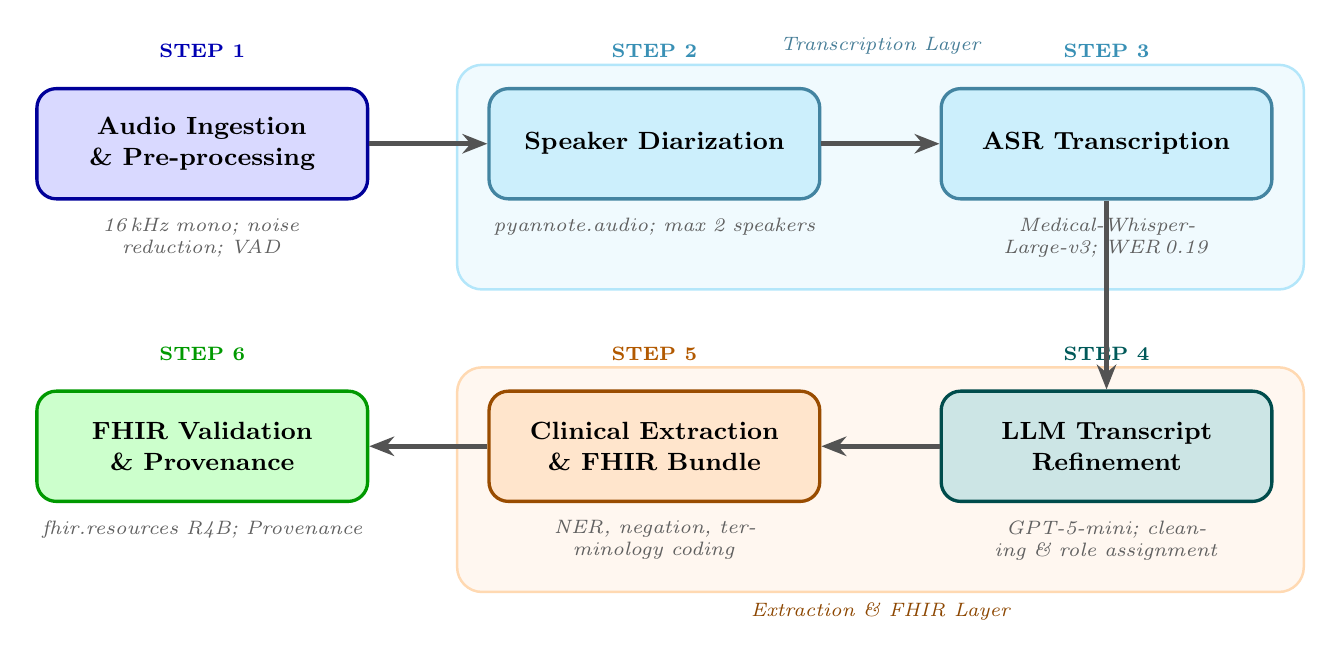
\begin{tikzpicture}[
    box/.style={
        rectangle, rounded corners=7pt,
        minimum width=4.2cm, minimum height=1.4cm,
        text centered, text width=3.9cm,
        font=\small\bfseries,
        line width=1.2pt
    },
    audio/.style ={box, fill=blue!15,   draw=blue!60!black},
    asr/.style   ={box, fill=cyan!20,   draw=cyan!60!black},
    llm/.style   ={box, fill=teal!20,   draw=teal!60!black},
    nlp/.style   ={box, fill=orange!20, draw=orange!60!black},
    fhir/.style  ={box, fill=green!20,  draw=green!60!black},
    sublabel/.style={
        font=\scriptsize\itshape,
        text=gray!75!black,
        text centered, text width=4.2cm
    },
    arr/.style={
        -{Stealth[length=9pt,width=7pt]},
        line width=1.8pt, color=gray!65!black
    },
    arrdown/.style={
        -{Stealth[length=9pt,width=7pt]},
        line width=1.8pt, color=gray!65!black,
        rounded corners=10pt
    },
]

% ROW 1
\node[audio] (step1) {Audio Ingestion \& Pre-processing};
\node[sublabel, below=0.10cm of step1] (step1-sub) {16\,kHz mono; noise reduction; VAD};

\node[asr, right=1.5cm of step1] (step2) {Speaker Diarization};
\node[sublabel, below=0.10cm of step2] (step2-sub) {pyannote.audio; max 2 speakers};

\node[asr, right=1.5cm of step2] (step3) {ASR Transcription};
\node[sublabel, below=0.10cm of step3] (step3-sub) {Medical-Whisper-Large-v3; WER\,0.19};

\node[font=\scriptsize\bfseries\color{blue!70!black},  above=0.25cm of step1] {STEP 1};
\node[font=\scriptsize\bfseries\color{cyan!70!black},  above=0.25cm of step2] {STEP 2};
\node[font=\scriptsize\bfseries\color{cyan!70!black},  above=0.25cm of step3] {STEP 3};

\draw[arr] (step1) -- (step2);
\draw[arr] (step2) -- (step3);

% ROW 2
\node[llm,  below=2.4cm of step3] (step4) {LLM Transcript Refinement};
\node[sublabel, below=0.10cm of step4] (step4-sub) {GPT-5-mini; cleaning \& role assignment};

\node[nlp, left=1.5cm of step4]   (step5) {Clinical Extraction \& FHIR Bundle};
\node[sublabel, below=0.10cm of step5] (step5-sub) {NER, negation, terminology coding};

\node[fhir, left=1.5cm of step5]  (step6) {FHIR Validation \& Provenance};
\node[sublabel, below=0.10cm of step6] (step6-sub) {fhir.resources R4B; Provenance};

\node[font=\scriptsize\bfseries\color{teal!70!black},   above=0.25cm of step4] {STEP 4};
\node[font=\scriptsize\bfseries\color{orange!70!black}, above=0.25cm of step5] {STEP 5};
\node[font=\scriptsize\bfseries\color{green!60!black},  above=0.25cm of step6] {STEP 6};

\draw[arr] (step4) -- (step5);
\draw[arr] (step5) -- (step6);

% Connecting arrow row1 -> row2
\draw[arrdown] (step3.south) -- ++(0,-0.9cm) -| (step4.north);

% Background shading
\begin{scope}[on background layer]
    \node[
        fill=cyan!6, draw=cyan!30, rounded corners=9pt, line width=0.9pt,
        fit=(step2)(step3)(step2-sub)(step3-sub),
        inner sep=8pt,
        label={[font=\scriptsize\itshape, text=cyan!55!black]above:Transcription Layer}
    ] {};

    \node[
        fill=orange!6, draw=orange!30, rounded corners=9pt, line width=0.9pt,
        fit=(step4)(step5)(step4-sub)(step5-sub),
        inner sep=8pt,
        label={[font=\scriptsize\itshape, text=orange!55!black]below:Extraction \& FHIR Layer}
    ] {};
\end{scope}

\end{tikzpicture}%
}% end resizebox

\caption{Overview of the proposed automated pipeline for mapping unstructured
clinical audio to HL7 FHIR-compliant data structures. The pipeline comprises
six sequential steps:
(1)~audio ingestion and pre-processing (16\,kHz resampling, noise reduction, voice activity detection);
(2)~speaker diarization via pyannote.audio constrained to two speakers~\cite{tran2022asr};
(3)~ASR transcription using Medical-Whisper-Large-v3~\cite{banerjee2024medasr};
(4)~LLM transcript refinement for cleaning and speaker role assignment~\cite{adedeji2024sound};
(5)~LLM clinical extraction producing a FHIR R4 Bundle via programmatic
\texttt{fhir.resources} construction~\cite{frei2025inferno};
and (6)~FHIR validation and provenance tracking~\cite{hl7fhir2022r4b}.}
\label{fig:pipeline}
\end{figure}




A central design decision is the collapse of the traditional multi-stage NLP pipeline — typically comprising SOAP segmentation, named entity recognition, negation detection, terminology normalization, and FHIR mapping as discrete components — into a single LLM extraction pass followed by schema-constrained, programmatic FHIR construction (Steps 5–6). This consolidation is motivated by Frei et al., who demonstrated a hallucination rate below 2.3\% when FHIR resources are assembled programmatically via \texttt{fhir.resources} object construction rather than generated as free-form JSON \cite{frei2025inferno}, and by Li et al., who demonstrated the feasibility of joint LLM-driven extraction and FHIR transformation \cite{li2024fhirgpt}.

All intermediate outputs are persisted to disk after each step (\path{outputs/<name>/step0N_<name>.json}). Completed steps are detected at startup and skipped, enabling iterative development and evaluation without full pipeline recomputation.

\subsection{Audio Ingestion and Pre-processing (Step 1)}

Step 1 accepts a single audio file and produces a pre-processed float32 waveform suitable for downstream ASR and diarization. The implementation uses three libraries: librosa ($\geq$0.10.2) for loading, noisereduce ($\geq$3.0.0) for stationary noise suppression, and webrtcvad-wheels for voice activity detection (VAD).

The processing sequence is as follows. The mixed audio file is loaded at 16,000\,Hz and downmixed to mono via librosa. Stationary background noise is suppressed using noisereduce's spectral subtraction method, which estimates a noise profile from nominally silent regions. Voice activity is then detected using WebRTC VAD, applied over non-overlapping 20\,ms frames (320 samples at 16\,kHz) at aggressiveness level 2 on the 0–3 scale. Frames classified as voiced are retained; the remainder are discarded. The output is an \texttt{IngestionResult} containing the voiced float32 array, sample rate, total duration, \textit{speech\_ratio} (voiced frames / total frames), and source path.

Empirically, speech\_ratio $\approx 0.55$ was observed on \texttt{day1\_consultation01\_doctor.wav} (457\,s total; approximately 250\,s voiced content). Filtering silence at this stage meaningfully reduces both ASR transcription time and the volume of non-speech segments passed to the diarization module.

\subsection{Automatic Speech Recognition (Steps 2--3)}

\subsubsection{Speaker Diarization (Step 2)}

Speaker diarization is performed using pyannote.audio 4.x \cite{tran2022asr} with the \path{pyannote/speaker-diarization-community-1} pre-trained model, executed on CPU. The pipeline is constrained to a maximum of two speakers, reflecting the doctor–patient consultation dyad. Output is a list of \texttt{Segment(start, end, speaker)} objects with generic labels \texttt{SPEAKER\_00} and \texttt{SPEAKER\_01}. Speaker role assignment — mapping generic labels to \textsc{physician} or \textsc{patient} — is deferred to Step 4, where the full transcript context is available to enable more accurate role inference. Independent evaluation of ASR systems on clinical dialogue has reported word-level diarization error rates (WDER) of 1.8–13.9\% under controlled conditions \cite{tran2022asr}, establishing a practical performance baseline for this component.

\subsubsection{ASR Transcription (Step 3)}

Transcription uses \path{Na0s/Medical-Whisper-Large-v3}, a 1.55B-parameter model fine-tuned on the PriMock57 training split by Banerjee et al.\ \cite{banerjee2024medasr}. The fine-tuned model achieves a word error rate of 0.19 on the PriMock57 validation split and 0.24 on the test split, representing a 42\% relative WER improvement over the zero-shot Whisper large-v3 baseline (WER 0.33) \cite{radford2023whisper}. The model is loaded via the HuggingFace \texttt{transformers} pipeline using \texttt{torch.float32} on CPU.

For each diarized segment of duration $\geq 0.1$\,s, the corresponding audio is sliced from the waveform using integer sample indices at 16\,kHz and passed to the ASR pipeline with \texttt{language="en"}. Each transcription is emitted as a \texttt{TranscriptSegment} (fields: start, end, speaker, text) carrying the diarization label. Segments shorter than 0.1\,s are discarded to avoid transcription artefacts from minimal audio content.

\subsection{LLM-Based Post-processing and Clinical Extraction (Steps 4--5)}

\subsubsection{Transcript Cleaning and Speaker Role Assignment (Step 4)}

Step 4 applies GPT-5-mini via the agno Agent framework with Pydantic-enforced structured output. A single LLM pass over the complete transcript simultaneously performs two tasks. First, transcription cleaning: filler words are removed, medical homophones are resolved (e.g.\ \textit{ileum} vs.\ \textit{ilium}), abbreviations are expanded (e.g.\ BP $\rightarrow$ blood pressure), and drug and anatomical names are corrected to standard spellings. Second, speaker role assignment: generic labels \texttt{SPEAKER\_00}/\texttt{SPEAKER\_01} are mapped to \textsc{physician} or \textsc{patient} based on full-transcript context, exploiting clinical questioning patterns, examination language, and symptom-reporting cues. The output schema is \texttt{\_LLMTranscript}, containing a list of \texttt{\_LLMSegment} (fields: index, speaker\_role, cleaned\_text).

Combining role assignment with transcript correction in a single LLM pass avoids a redundant API call and improves accuracy through access to global dialogue context \cite{efstathiadis2024diarization, adedeji2024sound}. The original ASR text is preserved in \texttt{PostProcessedSegment\discretionary{}{}{}.original\_text} for auditability and downstream error analysis.

\subsubsection{Clinical Extraction and FHIR Resource Generation (Step 5)}

Step 5 accepts the post-processed, role-labeled transcript and produces a validated FHIR R4 Bundle. The step uses GPT-5-mini via agno Agent with a Pydantic extraction schema, followed by programmatic FHIR construction via \texttt{fhir.resources}.

A single LLM pass jointly performs: named entity recognition across four resource types (Condition, MedicationStatement, Observation, Procedure); negation detection (e.g.\ ``no chest pain'' $\rightarrow$ \texttt{verificationStatus=refuted}; ``possible X'' $\rightarrow$ \texttt{unconfirmed}); relation extraction to capture drug–dose, route, and frequency as structured dosage fields; implicit SOAP classification (symptoms $\rightarrow$ unconfirmed Condition; examination/laboratory findings $\rightarrow$ Observation; diagnoses $\rightarrow$ confirmed Condition; plan items $\rightarrow$ MedicationStatement/Procedure); and best-effort terminology coding using SNOMED CT for conditions and procedures, RxNorm for medications, and LOINC for observations.

The LLM output is constrained to the following Pydantic schema:
\begin{itemize}
  \item \texttt{\_Condition}: text, clinical\_status, verification\_status, snomed\_code, icd10\_code, segment\_indices
  \item \texttt{\_Medication}: drug\_name, dose, route, frequency, status, rxnorm\_code, segment\_indices
  \item \texttt{\_Observation}: text, value, unit, loinc\_code, segment\_indices
  \item \texttt{\_Procedure}: text, status, snomed\_code, segment\_indices
\end{itemize}

FHIR R4 resources are then constructed programmatically via \texttt{fhir.resources} Pydantic models rather than as free-form JSON. The bundle includes Encounter, Condition, MedicationStatement, Observation, and Procedure resources, assembled as a collection-type Bundle. The Encounter period is derived from the minimum and maximum timestamps of transcript segments. Each resource carries a custom extension encoding \texttt{segment\_indices}, linking the resource back to its source transcript segments for auditability. Programmatic construction reduces the hallucination rate to below 2.3\% relative to free-form JSON generation \cite{frei2025inferno}.

This unified approach trades an accuracy ceiling — reported at 91\% semantic completeness and 0.88 interoperability for dedicated transformer-based NER pipelines with ontology-grounded normalization \cite{brens2025semantic} — for engineering simplicity and end-to-end pipeline integration. The trade-off is appropriate for a research prototype and consistent with the demonstrated feasibility of LLM-driven FHIR transformation in the literature \cite{hong2020nlp2fhir, li2024fhirgpt}.

\subsection{FHIR Validation and Provenance Tracking (Step 6)}

Step 6 performs structural validation of the generated bundle and attaches provenance metadata to each clinical resource. Both operations use \texttt{fhir.resources} Pydantic R4B models \cite{hl7fhir2022r4b}.

Validation parses each resource through its corresponding \texttt{fhir.resources} class (Condition, MedicationStatement, Observation, Procedure, Encounter, Bundle). Pydantic \texttt{ValidationError} exceptions are caught and converted to \texttt{ValidationIssue} records (fields: severity, resource\_type, resource\_id, message). The bundle is flagged \texttt{valid=True} if and only if no error-severity issues are raised; warning-severity issues are recorded but do not invalidate the bundle.

For each clinical resource, a FHIR \texttt{Provenance} resource is generated and appended to the bundle, carrying: a \texttt{target} reference to the clinical resource; a \texttt{recorded} timestamp of generation; an \texttt{agent.who} identifying the pipeline component (\path{rtm-pipeline/step05/gpt-5-mini}); an \texttt{entity.what} referencing the source audio filename; and a custom \texttt{nlp-system} extension valueString encoding the pipeline version. This approach follows the provenance extension conventions established by the SMART Text2FHIR pipeline \cite{miller2023smart}, enabling downstream consumers to reconstruct NLP provenance without rerunning the pipeline \cite{frei2025inferno}.

\subsection{Implementation Details}

The pipeline is implemented in Python 3.13, managed with uv. All inference is CPU-only: pyannote.audio and Whisper run on \texttt{device="cpu"} with \texttt{torch.float32}, with the ASR model requiring approximately 6\,GB of RAM for the 1.55B-parameter checkpoint. LLM calls are made to the OpenAI API (configured via the \texttt{OPENAI\_API\_KEY} environment variable); diarization model weights are retrieved from the HuggingFace Hub (configured via \texttt{HF\_TOKEN}). The runtime environment is NixOS, managed through devenv with direnv-based activation.


\bibliographystyle{plain}
%\bibliography{reference}

\begin{thebibliography}{99}

% --- ASR & Transcription ---

\bibitem{adedeji2024sound}
Ayo Adedeji, Sarita Joshi, and Brendan Doohan.
\newblock The sound of healthcare: Improving medical transcription {ASR}
  accuracy with large language models.
\newblock {\em arXiv preprint arXiv:2402.07658}, 2024.

\bibitem{banerjee2024medasr}
Sourav Banerjee, Ayushi Agarwal, and Promila Ghosh.
\newblock High-precision medical speech recognition through synthetic data and
  semantic correction: {United-MedASR}.
\newblock {\em arXiv preprint}, December 2024.

\bibitem{efstathiadis2024diarization}
Georgios Efstathiadis, Vijay Yadav, and Anzar Abbas.
\newblock {LLM}-based speaker diarization correction: A generalizable approach.
\newblock 2024.

\bibitem{klusty2024clinical}
Mitchell~A. Klusty, W.~Vaiden Logan, Samuel~E. Armstrong, Aaron~D. Mullen,
  Caroline~N. Leach, Ken Calvert, Jeff Talbert, and V.~K.~Cody Bumgardner.
\newblock Toward automated clinical transcriptions.
\newblock 2024.

\bibitem{papadopoulos2022primock57}
Alex {Papadopoulos Korfiatis}, Francesco Moramarco, Radmila Sarac, and
  Aleksandar Savkov.
\newblock {PriMock57}: A dataset of primary care mock consultations.
\newblock In {\em Proceedings of the Workshop on Clinical Natural Language
  Processing}, 2022.

\bibitem{radford2023whisper}
Alec Radford, Jong~Wook Kim, Tao Xu, Greg Brockman, Christine McLeavey, and
  Ilya Sutskever.
\newblock Robust speech recognition via large-scale weak supervision.
\newblock In {\em Proceedings of the 40th International Conference on Machine
  Learning ({ICML})}, 2023.

\bibitem{tran2022asr}
Brian~D. Tran, Ramya Mangu, Ming Tai-Seale, Jennifer~Elston Lafata, and
  Kai Zheng.
\newblock Automatic speech recognition performance for digital scribes: A
  performance comparison between general-purpose and specialized models tuned
  for patient-clinician conversations.
\newblock 2022.

% --- FHIR Resource Synthesis ---

\bibitem{frei2025inferno}
Johann Frei, Nils Feldhus, Lisa Raithel, Roland Roller, Alexander Meyer, and
  Frank Kramer.
\newblock Inferno: End-to-end agent-based {FHIR} resource synthesis from
  free-form clinical notes.
\newblock {\em arXiv preprint}, 2025.

\bibitem{hong2017integrating}
Na~Hong, Andrew Wen, Feichen Shen, Sunghwan Sohn, Sijia Liu, Hongfang Liu,
  and Guoqian Jiang.
\newblock Integrating structured and unstructured {EHR} data using an
  {FHIR}-based type system: A case study with medication data.
\newblock In {\em AMIA Annual Symposium Proceedings}, 2017.

\bibitem{hong2020nlp2fhir}
Na~Hong, Andrew Wen, Feichen Shen, Sunghwan Sohn, Chen Wang, Hongfang Liu,
  and Guoqian Jiang.
\newblock Developing a scalable {FHIR}-based clinical data normalization
  pipeline for standardizing and integrating unstructured and structured
  electronic health record data.
\newblock {\em Journal of the American Medical Informatics Association},
  2020.

\bibitem{li2024fhirgpt}
Yikuan Li, Hanyin Wang, Halid~Z. Yerebakan, Yoshihisa Shinagawa, and Yuan Luo.
\newblock {FHIR-GPT} enhances health interoperability with large language
  models.
\newblock {\em NEJM AI}, 1(8), August 2024.

\bibitem{miller2023smart}
Timothy~A. Miller, Andrew~J. McMurry, James Jones, Daniel Gottlieb, and
  Kenneth~D. Mandl.
\newblock The {SMART} {Text2FHIR} pipeline.
\newblock 2023.

\bibitem{riquelme2025llm}
{\'A}lvaro {Riquelme Tornel}, Pedro {Costa del Amo}, and Catalina
  {Mart{\'i}nez Costa}.
\newblock Large language models for automating structured clinical data
  standardization: {HL7 FHIR} use case.
\newblock 2025.

% --- Clinical NLP & LLMs ---

\bibitem{moldwin2021phenotyping}
Asher Moldwin, Dina Demner-Fushman, and Travis~R. Goodwin.
\newblock Empirical findings on the role of structured data, unstructured data,
  and their combination for automatic clinical phenotyping.
\newblock In {\em AMIA Annual Symposium Proceedings}, 2021.

\bibitem{brens2025semantic}
Rafael Brens, Yuqiao Meng, Luoxi Tang, and Zhaohan Xi.
\newblock Semantic {NLP} pipelines for interoperable patient digital twins from
  unstructured {EHR}s.
\newblock 2025.

\bibitem{builtjes2025leveraging}
Luc Builtjes, Joeran Bosma, Mathias Prokop, Bram {van Ginneken}, and
  Alessa Hering.
\newblock Leveraging open-source large language models for clinical information
  extraction in resource-constrained settings.
\newblock {\em Journal of the American Medical Informatics Association}, 2025.

\bibitem{saadat2025enhancing}
Saeed Saadat, Majid {Khalilizad Darounkolaei}, Mohsen Qorbani, Atefe Hemmat,
  and Sadaf Hariri.
\newblock Enhancing clinical documentation with {AI}: Reducing errors,
  improving interoperability, and supporting real-time note-taking.
\newblock {\em InfoScience Trends}, 2025.

% --- Standards ---

\bibitem{hl7fhir2022r4b}
{HL7 International}.
\newblock {HL7 FHIR} Release 4B (v4.3.0), 2022.
\newblock \url{https://hl7.org/fhir/R4B/}.

\end{thebibliography}


%USE THE BELOW OPTIONS IN CASE YOU NEED AUTHOR YEAR FORMAT.
%\bibliographystyle{abbrvnat}
%\bibliography{reference}


\end{document}
%%
%% Copyright 2021 OXFORD UNIVERSITY PRESS
%%
%% This file is part of the 'ima-authoring-template Bundle'.
%% ---------------------------------------------
%%
%% It may be distributed under the conditions of the LaTeX Project Public
%% License, either version 1.2 of this license or (at your option) any
%% later version.  The latest version of this license is in
%%    http://www.latex-project.org/lppl.txt
%% and version 1.2 or later is part of all distributions of LaTeX
%% version 1999/12/01 or later.
%%
%% The list of all files belonging to the 'ima-authoring-template Bundle' is
%% given in the file `manifest.txt'.
%%
%% Template article for OXFORD UNIVERSITY PRESS's document class `ima-authoring-template'
%% with bibliographic references
%%

\documentclass[webpdf, namedate]{ima-authoring-template}
%\documentclass[namedate,webpdf]{ima-authoring-template}

%\usepackage{showframe}

\usepackage[utf8]{inputenc}
\usepackage[T1]{fontenc}
\usepackage{url}
\usepackage{tikz}
\usepackage{geometry}
\usepackage{caption}
\usepackage{xurl}
\usepackage{microtype}

 \usetikzlibrary{arrows.meta, shapes.geometric, shapes.multipart, fit, positioning, backgrounds, shadows}

% \geometry{margin=1in}
\setlength{\emergencystretch}{10em}
\overfullrule=0pt

% line numbers
%\usepackage[mathlines, switch]{lineno}
%\usepackage[right]{lineno}

\theoremstyle{thmstyletwo}%
\newtheorem{theorem}{Theorem}%  meant for continuous numbers
%%\newtheorem{theorem}{Theorem}[section]% meant for sectionwise numbers
%% optional argument [theorem] produces theorem numbering sequence instead of independent numbers for Proposition
\newtheorem{proposition}[theorem]{Proposition}%
%%\newtheorem{proposition}{Proposition}% to get separate numbers for theorem and proposition etc.

\newtheorem{example}{Example}%
\newtheorem{remark}{Remark}%

\newtheorem{definition}{Definition}

\numberwithin{equation}{section}

\begin{document}

\DOI{DOI HERE}
\copyrightyear{2026}
\vol{00}
\pubyear{2026}
\access{Advance Access Publication Date: Day Month Year}
\appnotes{Paper}
% \copyrightstatement{Published by Oxford University Press on behalf of the Institute of Mathematics and its Applications. All rights reserved.}
\firstpage{1}

%\subtitle{Subject Section}

\title[Automated Clinical Audio-to-FHIR Pipeline]{Designing an Automated Pipeline for Mapping Unstructured Clinical Audio to HL7 FHIR-Compliant Data Structures}

\author{Dauren Baimurza*
\address{\orgdiv{Computer Science}, \orgname{SDU University}, \orgaddress{\street{Street}, \postcode{Postcode}, \state{Almaty}, \country{Kazakhstan}}}}
\authormark{Dauren Baimurza}

\corresp[*]{Corresponding author: \href{email:email-id.com}{email-id.com}}

\received{Date}{0}{Year}
\revised{Date}{0}{Year}
\accepted{Date}{0}{Year}

%\editor{Associate Editor: Name}


\abstract{Abstracts must be able to stand alone and so cannot contain citations to
the paper's references, equations, etc. An abstract must consist of a single
paragraph and be concise. Because of online formatting, abstracts must appear
as plain as possible.}
\keywords{Automatic Speech Recognition; Speaker Diarization; Clinical Audio Processing; Large Language Models; Clinical Information Extraction; HL7 FHIR; Healthcare Interoperability.}

% \boxedtext{
% \begin{itemize}
% \item Key boxed text here.
% \item Key boxed text here.
% \item Key boxed text here.
% \end{itemize}}



\maketitle



\section{Introduction}

\subsection{Background and Motivation}

The digitization of healthcare systems over the past two decades has led to exponential growth in the volume of clinical data generated across care settings. However, despite widespread adoption of Electronic Health Record (EHR) systems, a substantial proportion of clinically valuable information remains locked in unstructured formats — including physician dictations, bedside observations, referral notes, and patient-provider conversations. Studies have consistently demonstrated that unstructured data, when appropriately processed, contributes meaningfully to clinical tasks such as phenotyping and quality measurement, yet it remains largely inaccessible to automated systems in its raw form \cite{hong2020nlp2fhir}.

The coexistence of structured and unstructured data in healthcare presents both a challenge and an opportunity. Structured data — stored in coded fields and controlled vocabularies — enables systematic querying and analysis, while unstructured data often captures the richness, nuance, and context of clinical encounters that structured forms cannot convey \cite{hong2017integrating, brens2025semantic}. Empirical studies have quantified this complementarity: across 172 clinical phenotypes derived from MIMIC-III, textual features outperform structured measurements alone for 84\% of phenotypes, with their combination yielding statistically significant improvements for phenotypes where context recorded in clinical notes is not reflected in tabular measurements \cite{moldwin2021phenotyping}. Bridging this divide has long been recognized as a fundamental informatics challenge: extracting meaningful, computable representations from free-text and audio-based clinical content requires not only language understanding but also domain-specific knowledge and semantic reasoning \cite{builtjes2025leveraging}.

The scale of this documentation burden carries direct consequences for clinicians and patients alike. Primary care physicians spend a disproportionate share of their working time on administrative documentation rather than direct patient care — a pattern documented consistently across healthcare systems internationally \cite{saadat2025enhancing}. This imbalance is a well-established driver of clinician burnout, with documentation workload identified as one of the leading contributors to professional dissatisfaction and attrition \cite{klusty2024clinical}. Beyond the individual clinician, documentation delays introduce latency between clinical events and their representation in the EHR, undermining the timeliness of information available to care teams, degrading continuity of care, and increasing the risk of transcription error. Automating the transcription and structuring of clinical encounters therefore addresses not merely a technical inconvenience but a systemic inefficiency with measurable consequences for workforce sustainability, patient safety, and care quality. It is this imperative — reducing the manual overhead of clinical documentation while preserving its fidelity and interoperability — that motivates the present work.

Beyond text, clinical audio represents perhaps the most underutilized modality in health informatics. Encounters between patients and clinicians — whether in outpatient consultations, emergency settings, or telehealth platforms — generate continuous streams of spoken dialogue that contain diagnostically and clinically relevant content. The conversion of this audio into structured, actionable data remains overwhelmingly manual, relying on transcriptionists, clinical coders, or clinicians themselves to document encounters post hoc. This process is time-consuming, prone to inconsistency, and contributes significantly to the administrative burden placed on healthcare providers \cite{saadat2025enhancing, klusty2024clinical}.

\subsection{The Role of HL7 FHIR in Healthcare Interoperability}

HL7 Fast Healthcare Interoperability Resources (FHIR) has emerged as the leading international standard for the representation and exchange of healthcare information. By defining a modular, resource-based data model — encompassing clinical entities such as \texttt{Patient}, \texttt{Encounter}, \texttt{Observation}, \texttt{Condition}, and \texttt{MedicationRequest} — FHIR enables semantic interoperability across disparate health information systems \cite{hl7fhir2022r4b}. Recent work applying large language models to FHIR transformation has demonstrated a broad range of applications, including clinical decision support, patient data exchange, population health management, and regulatory reporting, while also highlighting persistent implementation challenges such as terminology binding, resource profiling complexity, and inconsistent adoption across jurisdictions \cite{li2024fhirgpt}.

The adoption of FHIR as a mandated or preferred interoperability standard by major healthcare regulators — including the U.S.\ Office of the National Coordinator for Health IT — has accelerated its uptake globally. Despite this progress, the vast majority of FHIR-compliant data structures are populated from existing structured EHR fields. The generation of FHIR resources from unstructured sources, particularly spoken clinical audio, remains an understudied and largely unsolved problem. Automating this pathway would not only reduce transcription burden but also enable real-time or near-real-time population of clinical records, supporting downstream analytics, care coordination, and research reuse.

\subsection{Automatic Speech Recognition in Healthcare}

Automatic Speech Recognition (ASR) technologies have undergone a paradigm shift in capability and accessibility, driven by deep learning architectures and large-scale pretraining. Radford et al.\ introduced Whisper, a general-purpose ASR model trained on 680,000 hours of multilingual, weakly supervised audio data, demonstrating near-human transcription accuracy and robust zero-shot generalization across diverse acoustic domains \cite{radford2023whisper}. The accessibility of such pretrained models makes them compelling candidates for integration into clinical audio processing pipelines, eliminating the need to train ASR systems from scratch.

The application of ASR in healthcare settings carries distinctive challenges that differentiate clinical speech from general-domain audio. Medical terminology is highly specialized, acoustically dense with domain-specific vocabulary (e.g., drug names, anatomical terms, diagnostic codes), and often produced under challenging recording conditions — background noise, overlapping speakers, and informal conversational register. Independent evaluation of both general-purpose and specialized ASR models on real patient-clinician conversations has confirmed that, even under controlled recording conditions, clinical dialogue yields word error rates of 8.8–10.5\% alongside variable speaker diarization accuracy \cite{tran2022asr}. The PriMock57 dataset — comprising 57 recorded mock primary care consultations with manual transcriptions — provides a key benchmark for evaluating ASR systems under realistic clinical dialogue conditions \cite{papadopoulos2022primock57}.

Recent work has explored the use of Large Language Models (LLMs) as post-processing layers to improve ASR output quality in medical transcription. Adedeji et al.\ demonstrated that applying LLMs — particularly through Chain-of-Thought (CoT) prompting — to refine ASR-generated transcripts of primary care consultations improved both general and medical-concept word error rates, while also enhancing speaker diarization accuracy and semantic coherence \cite{adedeji2024sound}. These findings collectively suggest that a hybrid pipeline — combining a pretrained ASR system with LLM-based post-processing — represents a practical and effective approach to medical transcription without requiring custom model development.

\subsection{From Transcription to Structured Clinical Data}

Transcription alone is insufficient for clinical informatics applications. To be computationally actionable, spoken clinical content must be transformed into structured representations grounded in standard terminologies and data models. This requires NLP pipelines capable of named entity recognition, relation extraction, negation detection, and normalization against controlled vocabularies such as SNOMED CT, LOINC, and RxNorm. The extraction of clinical information from unstructured data — including clinical notes and transcribed encounters — has been demonstrated as feasible using open-source LLMs in zero-shot settings, though accuracy varies substantially by entity type and documentation style \cite{builtjes2025leveraging}.

Mapping extracted clinical concepts to FHIR resources introduces an additional layer of complexity. Each FHIR resource type carries specific structural requirements, terminology bindings, and cardinality constraints that must be satisfied to produce conformant output. The challenge of designing a pipeline that traverses the full pathway from raw audio to validated FHIR resource instances — integrating ASR, NLP, terminology normalization, and resource generation — has not been comprehensively addressed in the literature. Existing approaches tend to address individual stages in isolation, leaving the end-to-end integration as an open engineering and research problem \cite{hong2020nlp2fhir, riquelme2025llm}.

\subsection{Problem Statement}

Despite the individual maturity of its constituent technologies — ASR, clinical NLP, and FHIR modelling — no established solution integrates these into a coherent, end-to-end pipeline that transforms raw clinical audio into validated, interoperable FHIR resources. Existing approaches address individual stages in isolation: ASR systems are evaluated for transcription accuracy without downstream clinical structuring; NLP pipelines operate on pre-existing text rather than live transcriptions; and FHIR generation tools assume structured or semi-structured input rather than conversational speech. The resulting fragmentation means that the full pathway from an audio recording of a clinical encounter to a computable, standards-conformant clinical record remains an open engineering and research problem \cite{hong2020nlp2fhir, riquelme2025llm}.

This study therefore poses the following question: can an automated pipeline — built from existing pretrained components — reliably transcribe primary care consultations and produce clinically meaningful, FHIR R4B-conformant resources, without requiring custom model development or manual post-editing?

\subsection{Research Objectives and Scope}

This study presents the design and evaluation of an automated pipeline for mapping unstructured clinical audio to HL7 FHIR Release 4B-compliant data structures \cite{hl7fhir2022r4b}. Rather than developing novel ASR or NLP models from scratch, the proposed system integrates and orchestrates existing pretrained components — including Whisper \cite{radford2023whisper} for transcription and LLM-based processing for clinical entity identification \cite{adedeji2024sound} — within a unified, modular architecture. The pipeline is developed and evaluated using the PriMock57 dataset of primary care mock consultations \cite{papadopoulos2022primock57}. By utilizing a dataset consisting of mock consultations with professional actors, this research minimizes ethical risks associated with the exposure of sensitive patient-identifiable information while maintaining clinical realism. The novelty of this work lies in the pipeline design itself: specifically, the systematic integration of these components, the application of LLM-driven post-processing for both transcription refinement and clinical information extraction, and the mapping of extracted entities to validated FHIR resource structures.

The remainder of this paper is organized as follows. Section~2 reviews related work spanning clinical ASR, medical NLP, and FHIR-based data modeling. Section~3 describes the proposed pipeline architecture and its constituent components. Section~4 details the experimental setup and evaluation methodology. Section~5 presents results and discussion, and Section~6 concludes with implications for clinical practice and directions for future research.






\section{Literature Review}

\subsection{Clinical Documentation Burden and AI-Assisted Transcription}
Administrative documentation is a leading driver of clinician burnout and reduced care quality. Manual note-taking during consultations is time-consuming, error-prone, and diverts clinician attention from the patient. Systems that combine automatic speech recognition (ASR) with speaker diarization offer a path toward automated, speaker-labeled clinical transcripts, significantly reducing the documentation burden \cite{klusty2024clinical, saadat2025enhancing}.

Systematic reviews of AI-assisted clinical documentation show that integrating NLP, ASR, and large language models (LLMs) reduces transcription errors, supports real-time note generation via SOAP templates, and improves EHR interoperability. Techniques such as ClinicalBERT and GPT-4 fine-tuning, alongside hybrid extractive-abstractive summarization, have been demonstrated to accelerate structured note generation. Key limitations remain, however: hallucination risk and low clinician trust continue to hinder adoption \cite{saadat2025enhancing}.

Open-source generative LLMs—including Llama-3.3-70B, Phi-4-14B, and Qwen-2.5-14B—have been evaluated in zero-shot settings for clinical information extraction from medical texts. These models demonstrate strong performance, matching or exceeding fine-tuned RoBERTa baselines on structured inference tasks. Importantly, native-language processing must be preserved; translation to English consistently degrades extraction quality, underscoring the importance of multilingual model support \cite{builtjes2025leveraging}.

\subsection{Automatic Speech Recognition for Clinical Speech}
Radford et al.\ introduced Whisper, a general-purpose ASR system trained on 680,000 hours of weakly supervised multilingual audio. Its zero-shot performance approaches human-level accuracy across diverse acoustic conditions, making it a compelling foundation for clinical pipelines that cannot rely on large labeled datasets \cite{radford2023whisper}.

Independent evaluation of general-purpose and medical-specialized ASR systems on 36 patient-clinician conversations reports word error rates (WER) of 8.8–10.5\% and word-level diarization error rates (WDER) of 1.8–13.9\% under controlled recording conditions. Counterintuitively, general-purpose models sometimes outperform medical-specialized variants on diarization accuracy. Medical concept recall (F-recall \textasciitilde{}0.48–0.49) remains low despite high transcription precision, motivating further LLM post-processing stages \cite{tran2022asr}.

To address domain-specific terminology gaps, United-MedASR layers a BART-based semantic correction model over Faster Whisper, fine-tuned on synthetic vocabulary derived from ICD-10, MIMS, and FDA databases. This approach achieves WER below 1\% on benchmark corpora without requiring private patient data, demonstrating that synthetic domain adaptation is a viable and privacy-preserving strategy \cite{banerjee2024medasr}.

PriMock57 provides 57 mock primary care consultations with manual utterance-level transcriptions and consultation notes, representing one of the few publicly available clinical audio benchmarks due to stringent privacy constraints. It enables reproducible evaluation of ASR and note-generation systems and serves as the evaluation corpus for this study \cite{papadopoulos2022primock57}.

Diarization accuracy is sensitive to audio quality, overlapping speech, and the choice of ASR tool. Fine-tuned LLMs applied as a post-processing layer can markedly improve diarization accuracy; however, models fine-tuned on one ASR system's outputs underperform when applied to others, motivating ensemble approaches. LLM post-processing with chain-of-thought (CoT) prompting further improves medical-concept WER and speaker role assignment in primary care transcripts \cite{efstathiadis2024diarization, adedeji2024sound}.

\subsection{Clinical Information Extraction and NLP Pipelines}
Empirical comparison of structured and unstructured EHR data for automatic clinical phenotyping reveals that textual features — encoded via Doc2Vec — outperform structured measurements alone for 84\% of 172 clinical phenotypes from MIMIC-III, with Doc2Vec consistently dominating Bag-of-Words and Bag-of-Concepts representations. Combining structured data with Doc2Vec-encoded clinical notes yields statistically significant AUC improvements for 51 phenotypes, particularly in the circulatory system and injury/poisoning categories, where radiology and surgical report context is diagnostically decisive. For a single phenotype (diabetes without complications), structured data alone performs better, confirming that phenotype-specific data source selection remains important. These findings establish a clear empirical basis for multimodal pipelines that fuse structured and unstructured clinical data \cite{moldwin2021phenotyping}.

Hong et al.\ introduced a FHIR-based type system enabling integration of structured and unstructured EHR data via UIMA-based NLP tools (MedXN, MedTime). A case study on medication data from Mayo Clinic's EHR achieved F-scores of 0.73–0.99 across FHIR element representations, demonstrating the feasibility of standards-based NLP pipelines for clinical information extraction \cite{hong2017integrating}.

Building on this foundation, the NLP2FHIR pipeline extends FHIR-based normalization into a scalable framework implementing 30 mapping rules, 62 normalization rules, and 11 FHIR extensions to handle Condition, Procedure, MedicationStatement, and FamilyMemberHistory resources from Mayo Clinic unstructured EHRs. F-scores ranging from 0.69–0.99 confirm the feasibility of FHIR-compliant modeling at scale \cite{hong2020nlp2fhir}.

More recently, transformer-based NER combined with ontology-grounded concept normalization (SNOMED-CT, ICD-10, RxNorm, LOINC) and relation extraction has been shown to produce FHIR-compliant patient digital twin representations from free-text clinical narratives. Evaluation on MIMIC-IV Demo achieves 0.89 NER F1, 0.81 relation extraction F1, 91\% semantic completeness, and an interoperability score of 0.88. Concept normalization is identified as the single factor with the highest isolated impact on overall interoperability \cite{brens2025semantic}.

\subsection{FHIR-Based Interoperability and LLM-Driven Resource Synthesis}
HL7 FHIR Release 4B defines a modular, resource-based data model adopted by major healthcare regulators globally. Its RESTful architecture and emphasis on implementability have driven broad adoption across EHR vendors and research platforms, making it the de facto standard for clinical data exchange \cite{hl7fhir2022r4b}.

FHIR-GPT demonstrates that LLMs can convert clinical narratives into FHIR medication statements with greater than 90\% exact match rate, outperforming dedicated rule-based NLP pipelines by 3–50\% across attributes such as route, dose, reason, form, and timing. This confirms that LLMs can effectively replace modular NLP pipelines for FHIR transformation tasks while remaining more flexible to varied input formats \cite{li2024fhirgpt}.

The Inferno framework advances this direction by using LLM agents equipped with SNOMED CT tools and code execution to synthesize FHIR resources from discharge letters, competing with a human baseline. Programmatic FHIR object construction via the \texttt{fhir.resources} library, rather than free-form JSON generation, reduces hallucination rates to below 2.3\%, illustrating the value of structured output constraints in agentic pipelines \cite{frei2025inferno}.

The SMART Text2FHIR pipeline demonstrates an NLP-centric alternative, using Apache cTAKES to extract clinical concepts from EHR notes and map them to FHIR Observation, Condition, Procedure, and MedicationStatement resources, with extensions for negation, NLP sourcing, and provenance. Increased FHIR data liquidity driven by interoperability regulations makes such NLP-to-FHIR pipelines viable at institutional scale \cite{miller2023smart}.

Finally, retrieval-augmented generation (RAG)-enhanced LLMs—including GPT-4o and Llama 3.2 405B—applied to MIMIC-IV structured data achieve 67–73\% attribute-level FHIR mapping accuracy. Detailed JSON schemas and semantic clustering help narrow ambiguity, while iterative prompting further refines outputs. Persistent challenges include model hallucinations and incomplete source field descriptions, highlighting the continued need for validation layers in automated FHIR generation pipelines \cite{riquelme2025llm}.

\subsection{Critical Synthesis and Research Gap}

Reviewed works collectively advance the constituent technologies of clinical audio-to-FHIR pipelines, yet several systemic weaknesses recur across the literature and directly motivate the present study.

\textbf{Fragmentation across pipeline stages.} Existing work treats ASR, clinical NLP, and FHIR generation as isolated research problems rather than as interdependent stages of a single system. ASR studies evaluate transcription quality in isolation without propagating errors to downstream structuring tasks \cite{tran2022asr, radford2023whisper, adedeji2024sound}. NLP-to-FHIR pipelines assume clean text input, side-stepping the speech recognition and diarisation errors that would arise in real deployment \cite{hong2020nlp2fhir, brens2025semantic, miller2023smart}. FHIR synthesis systems similarly presuppose structured or semi-structured input \cite{li2024fhirgpt, frei2025inferno, riquelme2025llm}. No prior work evaluates the cumulative effect of chaining these stages, leaving the error amplification across the full pipeline unmeasured.

\textbf{Input assumptions that disconnect from clinical reality.} Text-to-FHIR pipelines are evaluated on pre-existing EHR notes: NLP2FHIR operates on Mayo Clinic records \cite{hong2020nlp2fhir}, Inferno on discharge letters \cite{frei2025inferno}, and SMART Text2FHIR on cTAKES-processed notes \cite{miller2023smart}. These inputs are already partially structured and free of ASR noise. A real clinical deployment must handle raw conversational audio with overlapping speakers, informal register, and domain-specific terminology — challenges none of the FHIR-generation studies address.

\textbf{Narrow evaluation scope and proprietary data.} Most FHIR generation studies target a limited resource subset: FHIR-GPT focuses on medication statements \cite{li2024fhirgpt} and Inferno on discharge-letter entities \cite{frei2025inferno}. Reproducibility is further constrained by reliance on proprietary datasets such as the Mayo Clinic EHR or MIMIC-IV under restricted access. The 67–73\% attribute-level accuracy reported for RAG-enhanced LLMs \cite{riquelme2025llm} illustrates that even state-of-the-art approaches leave a substantial accuracy gap — and this figure is obtained on clean structured input, not upstream ASR output.

\textbf{Lack of end-to-end conformance validation.} Hallucination and conformance errors persist across reviewed systems: Inferno reports hallucination rates below 2.3\% only after applying constrained programmatic FHIR construction \cite{frei2025inferno}, while Riquelme et al.\ note persistent incomplete field mappings despite iterative prompting \cite{riquelme2025llm}. No reviewed study performs full HL7 FHIR R4B conformance validation on pipeline output derived from spoken audio.

These gaps collectively motivate a unified pipeline that: (a) begins from raw audio rather than pre-existing text, (b) integrates ASR, diarisation, LLM post-processing, clinical NLP, and FHIR generation as a single evaluated system, (c) uses PriMock57 — a public, realistic clinical audio benchmark \cite{papadopoulos2022primock57} — to ensure reproducibility, and (d) includes HL7 FHIR R4B conformance validation as a first-class evaluation criterion.




\section{Methodology}

\subsection{Dataset}

The PriMock57 dataset \cite{papadopoulos2022primock57} consists of 57 mock primary care consultations recorded over five days by clinicians at Babylon Health. The corpus comprises 114 mono WAV audio files: a separate doctor track and a separate patient track per consultation, named according to the convention \path{dayN_consultationNN_role.wav}, where \textit{N} indexes the recording day (1–5) and \textit{role} is \texttt{doctor} or \texttt{patient}. Ground-truth annotations include manual utterance-level transcriptions and consultation notes produced by the recording clinicians. PriMock57 is, to our knowledge, the only publicly available clinical audio benchmark with ground-truth transcripts at the consultation level, making it the natural evaluation corpus for end-to-end audio-to-FHIR research.

Prior to pipeline ingestion, the two per-consultation tracks are mixed via additive synthesis: the doctor and patient waveforms are loaded at the same sample rate, summed sample-by-sample, and peak-normalized to amplitude 1.0. This yields a single-channel recording that simulates a room-microphone capture of the consultation dyad. An optional 60-second trim was applied to individual consultations during development to accelerate iterative testing.

\subsection{Pipeline Architecture}

The system is organized as a six-step pipeline spanning four functional phases: (1) acoustic pre-processing, (2) automatic speech recognition with speaker attribution, (3) LLM-driven transcript refinement and clinical information extraction, and (4) FHIR resource generation with validation and provenance tracking. The six steps are illustrated in Figure~\ref{fig:pipeline}.

\begin{enumerate}
  \item Audio Ingestion \& Pre-processing
  \item Speaker Diarization
  \item ASR Transcription
  \item LLM Transcript Cleaning \& Speaker Role Assignment
  \item LLM Clinical Extraction \textrightarrow{} FHIR R4 Bundle Construction
  \item FHIR Validation \& Provenance Tracking
\end{enumerate}



\begin{figure}[ht]
\centering
\resizebox{\linewidth}{!}{%
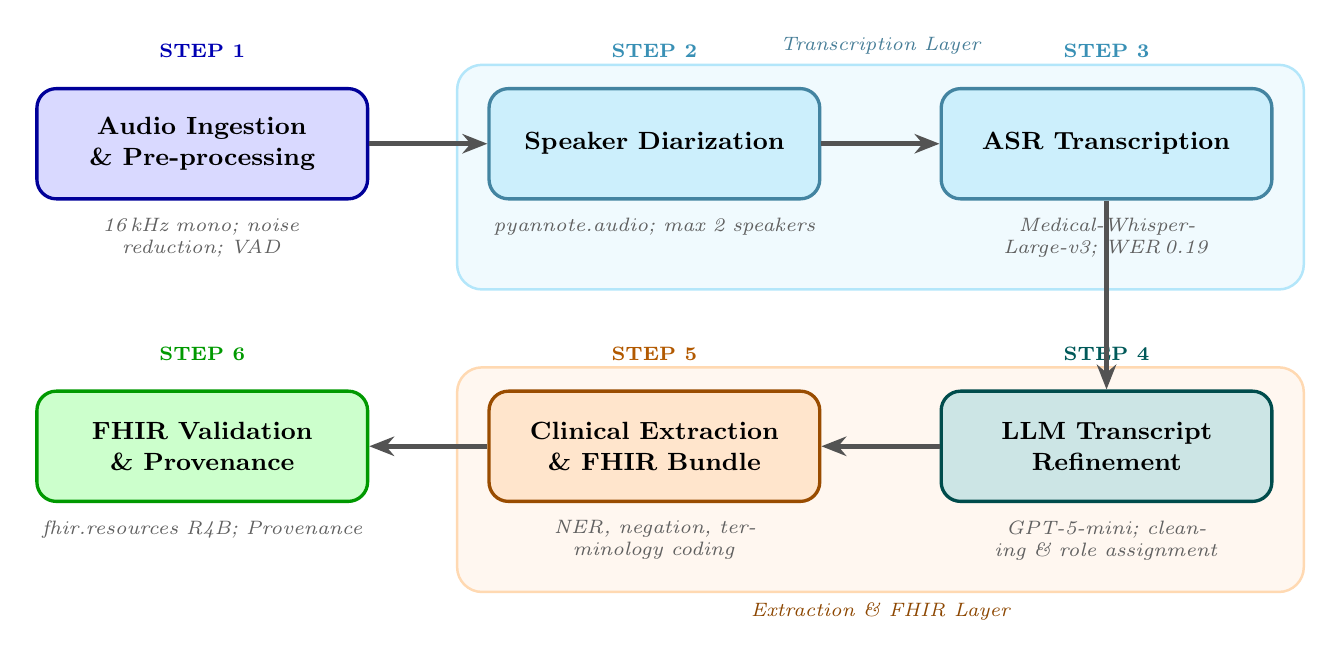
\begin{tikzpicture}[
    box/.style={
        rectangle, rounded corners=7pt,
        minimum width=4.2cm, minimum height=1.4cm,
        text centered, text width=3.9cm,
        font=\small\bfseries,
        line width=1.2pt
    },
    audio/.style ={box, fill=blue!15,   draw=blue!60!black},
    asr/.style   ={box, fill=cyan!20,   draw=cyan!60!black},
    llm/.style   ={box, fill=teal!20,   draw=teal!60!black},
    nlp/.style   ={box, fill=orange!20, draw=orange!60!black},
    fhir/.style  ={box, fill=green!20,  draw=green!60!black},
    sublabel/.style={
        font=\scriptsize\itshape,
        text=gray!75!black,
        text centered, text width=4.2cm
    },
    arr/.style={
        -{Stealth[length=9pt,width=7pt]},
        line width=1.8pt, color=gray!65!black
    },
    arrdown/.style={
        -{Stealth[length=9pt,width=7pt]},
        line width=1.8pt, color=gray!65!black,
        rounded corners=10pt
    },
]

% ROW 1
\node[audio] (step1) {Audio Ingestion \& Pre-processing};
\node[sublabel, below=0.10cm of step1] (step1-sub) {16\,kHz mono; noise reduction; VAD};

\node[asr, right=1.5cm of step1] (step2) {Speaker Diarization};
\node[sublabel, below=0.10cm of step2] (step2-sub) {pyannote.audio; max 2 speakers};

\node[asr, right=1.5cm of step2] (step3) {ASR Transcription};
\node[sublabel, below=0.10cm of step3] (step3-sub) {Medical-Whisper-Large-v3; WER\,0.19};

\node[font=\scriptsize\bfseries\color{blue!70!black},  above=0.25cm of step1] {STEP 1};
\node[font=\scriptsize\bfseries\color{cyan!70!black},  above=0.25cm of step2] {STEP 2};
\node[font=\scriptsize\bfseries\color{cyan!70!black},  above=0.25cm of step3] {STEP 3};

\draw[arr] (step1) -- (step2);
\draw[arr] (step2) -- (step3);

% ROW 2
\node[llm,  below=2.4cm of step3] (step4) {LLM Transcript Refinement};
\node[sublabel, below=0.10cm of step4] (step4-sub) {GPT-5-mini; cleaning \& role assignment};

\node[nlp, left=1.5cm of step4]   (step5) {Clinical Extraction \& FHIR Bundle};
\node[sublabel, below=0.10cm of step5] (step5-sub) {NER, negation, terminology coding};

\node[fhir, left=1.5cm of step5]  (step6) {FHIR Validation \& Provenance};
\node[sublabel, below=0.10cm of step6] (step6-sub) {fhir.resources R4B; Provenance};

\node[font=\scriptsize\bfseries\color{teal!70!black},   above=0.25cm of step4] {STEP 4};
\node[font=\scriptsize\bfseries\color{orange!70!black}, above=0.25cm of step5] {STEP 5};
\node[font=\scriptsize\bfseries\color{green!60!black},  above=0.25cm of step6] {STEP 6};

\draw[arr] (step4) -- (step5);
\draw[arr] (step5) -- (step6);

% Connecting arrow row1 -> row2
\draw[arrdown] (step3.south) -- ++(0,-0.9cm) -| (step4.north);

% Background shading
\begin{scope}[on background layer]
    \node[
        fill=cyan!6, draw=cyan!30, rounded corners=9pt, line width=0.9pt,
        fit=(step2)(step3)(step2-sub)(step3-sub),
        inner sep=8pt,
        label={[font=\scriptsize\itshape, text=cyan!55!black]above:Transcription Layer}
    ] {};

    \node[
        fill=orange!6, draw=orange!30, rounded corners=9pt, line width=0.9pt,
        fit=(step4)(step5)(step4-sub)(step5-sub),
        inner sep=8pt,
        label={[font=\scriptsize\itshape, text=orange!55!black]below:Extraction \& FHIR Layer}
    ] {};
\end{scope}

\end{tikzpicture}%
}% end resizebox

\caption{Overview of the proposed automated pipeline for mapping unstructured
clinical audio to HL7 FHIR-compliant data structures. The pipeline comprises
six sequential steps:
(1)~audio ingestion and pre-processing (16\,kHz resampling, noise reduction, voice activity detection);
(2)~speaker diarization via pyannote.audio constrained to two speakers~\cite{tran2022asr};
(3)~ASR transcription using Medical-Whisper-Large-v3~\cite{banerjee2024medasr};
(4)~LLM transcript refinement for cleaning and speaker role assignment~\cite{adedeji2024sound};
(5)~LLM clinical extraction producing a FHIR R4 Bundle via programmatic
\texttt{fhir.resources} construction~\cite{frei2025inferno};
and (6)~FHIR validation and provenance tracking~\cite{hl7fhir2022r4b}.}
\label{fig:pipeline}
\end{figure}




A central design decision is the collapse of the traditional multi-stage NLP pipeline — typically comprising SOAP segmentation, named entity recognition, negation detection, terminology normalization, and FHIR mapping as discrete components — into a single LLM extraction pass followed by schema-constrained, programmatic FHIR construction (Steps 5–6). This consolidation is motivated by Frei et al., who demonstrated a hallucination rate below 2.3\% when FHIR resources are assembled programmatically via \texttt{fhir.resources} object construction rather than generated as free-form JSON \cite{frei2025inferno}, and by Li et al., who demonstrated the feasibility of joint LLM-driven extraction and FHIR transformation \cite{li2024fhirgpt}.

All intermediate outputs are persisted to disk after each step (\path{outputs/<name>/step0N_<name>.json}). Completed steps are detected at startup and skipped, enabling iterative development and evaluation without full pipeline recomputation.

\subsection{Audio Ingestion and Pre-processing (Step 1)}

Step 1 accepts a single audio file and produces a pre-processed float32 waveform suitable for downstream ASR and diarization. The implementation uses three libraries: librosa ($\geq$0.10.2) for loading, noisereduce ($\geq$3.0.0) for stationary noise suppression, and webrtcvad-wheels for voice activity detection (VAD).

The processing sequence is as follows. The mixed audio file is loaded at 16,000\,Hz and downmixed to mono via librosa. Stationary background noise is suppressed using noisereduce's spectral subtraction method, which estimates a noise profile from nominally silent regions. Voice activity is then detected using WebRTC VAD, applied over non-overlapping 20\,ms frames (320 samples at 16\,kHz) at aggressiveness level 2 on the 0–3 scale. Frames classified as voiced are retained; the remainder are discarded. The output is an \texttt{IngestionResult} containing the voiced float32 array, sample rate, total duration, \textit{speech\_ratio} (voiced frames / total frames), and source path.

Empirically, speech\_ratio $\approx 0.85$ was observed on \texttt{day1\_consultation01\_mixed.wav} (387\,s total; approximately 328\,s voiced content). Filtering silence at this stage meaningfully reduces both ASR transcription time and the volume of non-speech segments passed to the diarization module.
2
\subsection{Automatic Speech Recognition (Steps 2--3)}

\subsubsection{Speaker Diarization (Step 2)}

Speaker diarization is performed using pyannote.audio 4.x \cite{tran2022asr} with the \path{pyannote/speaker-diarization-community-1} pre-trained model, executed on CPU. The pipeline is constrained to a maximum of two speakers, reflecting the doctor–patient consultation dyad. Output is a list of \texttt{Segment(start, end, speaker)} objects with generic labels \texttt{SPEAKER\_00} and \texttt{SPEAKER\_01}. Speaker role assignment — mapping generic labels to \textsc{physician} or \textsc{patient} — is deferred to Step 4, where the full transcript context is available to enable more accurate role inference. Independent evaluation of ASR systems on clinical dialogue has reported word-level diarization error rates (WDER) of 1.8–13.9\% under controlled conditions \cite{tran2022asr}, establishing a practical performance baseline for this component.

\subsubsection{ASR Transcription (Step 3)}

Transcription uses \path{Na0s/Medical-Whisper-Large-v3}, a 1.55B-parameter model fine-tuned on the PriMock57 training split by Banerjee et al.\ \cite{banerjee2024medasr}. The fine-tuned model achieves a word error rate of 0.19 on the PriMock57 validation split and 0.24 on the test split, representing a 42\% relative WER improvement over the zero-shot Whisper large-v3 baseline (WER 0.33) \cite{radford2023whisper}. The model is loaded via the HuggingFace \texttt{transformers} pipeline using \texttt{torch.float32} on CPU.

For each diarized segment of duration $\geq 0.1$\,s, the corresponding audio is sliced from the waveform using integer sample indices at 16\,kHz and passed to the ASR pipeline with \texttt{language="en"}. Each transcription is emitted as a \texttt{TranscriptSegment} (fields: start, end, speaker, text) carrying the diarization label. Segments shorter than 0.1\,s are discarded to avoid transcription artefacts from minimal audio content.

\subsection{LLM-Based Post-processing and Clinical Extraction (Steps 4--5)}

\subsubsection{Transcript Cleaning and Speaker Role Assignment (Step 4)}

Step 4 applies GPT-5-mini via the agno Agent framework with Pydantic-enforced structured output. A single LLM pass over the complete transcript simultaneously performs two tasks. First, transcription cleaning: filler words are removed, medical homophones are resolved (e.g.\ \textit{ileum} vs.\ \textit{ilium}), abbreviations are expanded (e.g.\ BP $\rightarrow$ blood pressure), and drug and anatomical names are corrected to standard spellings. Second, speaker role assignment: generic labels \texttt{SPEAKER\_00}/\texttt{SPEAKER\_01} are mapped to \textsc{physician} or \textsc{patient} based on full-transcript context, exploiting clinical questioning patterns, examination language, and symptom-reporting cues. The output schema is \texttt{\_LLMTranscript}, containing a list of \texttt{\_LLMSegment} (fields: index, speaker\_role, cleaned\_text).

Combining role assignment with transcript correction in a single LLM pass avoids a redundant API call and improves accuracy through access to global dialogue context \cite{efstathiadis2024diarization, adedeji2024sound}. The original ASR text is preserved in \texttt{PostProcessedSegment\discretionary{}{}{}.original\_text} for auditability and downstream error analysis.

\subsubsection{Clinical Extraction and FHIR Resource Generation (Step 5)}

Step 5 accepts the post-processed, role-labeled transcript and produces a validated FHIR R4 Bundle. The step uses GPT-5-mini via agno Agent with a Pydantic extraction schema, followed by programmatic FHIR construction via \texttt{fhir.resources}.

A single LLM pass jointly performs: named entity recognition across four resource types (Condition, MedicationStatement, Observation, Procedure); negation detection (e.g.\ ``no chest pain'' $\rightarrow$ \texttt{verificationStatus=refuted}; ``possible X'' $\rightarrow$ \texttt{unconfirmed}); relation extraction to capture drug–dose, route, and frequency as structured dosage fields; implicit SOAP classification (symptoms $\rightarrow$ unconfirmed Condition; examination/laboratory findings $\rightarrow$ Observation; diagnoses $\rightarrow$ confirmed Condition; plan items $\rightarrow$ MedicationStatement/Procedure); and best-effort terminology coding using SNOMED CT for conditions and procedures, RxNorm for medications, and LOINC for observations.

The LLM output is constrained to the following Pydantic schema:
\begin{itemize}
  \item \texttt{\_Condition}: text, clinical\_status, verification\_status, snomed\_code, icd10\_code, segment\_indices
  \item \texttt{\_Medication}: drug\_name, dose, route, frequency, status, rxnorm\_code, segment\_indices
  \item \texttt{\_Observation}: text, value, unit, loinc\_code, segment\_indices
  \item \texttt{\_Procedure}: text, status, snomed\_code, segment\_indices
\end{itemize}

FHIR R4 resources are then constructed programmatically via \texttt{fhir.resources} Pydantic models rather than as free-form JSON. The bundle includes Encounter, Condition, MedicationStatement, Observation, and Procedure resources, assembled as a collection-type Bundle. The Encounter period is derived from the minimum and maximum timestamps of transcript segments. Each resource carries a custom extension encoding \texttt{segment\_indices}, linking the resource back to its source transcript segments for auditability. Programmatic construction reduces the hallucination rate to below 2.3\% relative to free-form JSON generation \cite{frei2025inferno}.

This unified approach trades an accuracy ceiling — reported at 91\% semantic completeness and 0.88 interoperability for dedicated transformer-based NER pipelines with ontology-grounded normalization \cite{brens2025semantic} — for engineering simplicity and end-to-end pipeline integration. The trade-off is appropriate for a research prototype and consistent with the demonstrated feasibility of LLM-driven FHIR transformation in the literature \cite{hong2020nlp2fhir, li2024fhirgpt}.

\subsection{FHIR Validation and Provenance Tracking (Step 6)}

Step 6 performs structural validation of the generated bundle and attaches provenance metadata to each clinical resource. Both operations use \texttt{fhir.resources} Pydantic R4B models \cite{hl7fhir2022r4b}.

Validation parses each resource through its corresponding \texttt{fhir.resources} class (Condition, MedicationStatement, Observation, Procedure, Encounter, Bundle). Pydantic \texttt{ValidationError} exceptions are caught and converted to \texttt{ValidationIssue} records (fields: severity, resource\_type, resource\_id, message). The bundle is flagged \texttt{valid=True} if and only if no error-severity issues are raised; warning-severity issues are recorded but do not invalidate the bundle.

For each clinical resource, a FHIR \texttt{Provenance} resource is generated and appended to the bundle, carrying: a \texttt{target} reference to the clinical resource; a \texttt{recorded} timestamp of generation; an \texttt{agent.who} identifying the pipeline component (\path{rtm-pipeline/step05/gpt-5-mini}); an \texttt{entity.what} referencing the source audio filename; and a custom \texttt{nlp-system} extension valueString encoding the pipeline version. This approach follows the provenance extension conventions established by the SMART Text2FHIR pipeline \cite{miller2023smart}, enabling downstream consumers to reconstruct NLP provenance without rerunning the pipeline \cite{frei2025inferno}.

\subsection{Implementation Details}

The pipeline is implemented in Python 3.13, managed with uv. All inference is CPU-only: pyannote.audio and Whisper run on \texttt{device="cpu"} with \texttt{torch.float32}, with the ASR model requiring approximately 6\,GB of RAM for the 1.55B-parameter checkpoint. LLM calls are made to the OpenAI API (configured via the \texttt{OPENAI\_API\_KEY} environment variable); diarization model weights are retrieved from the HuggingFace Hub (configured via \texttt{HF\_TOKEN}). The runtime environment is NixOS, managed through devenv with direnv-based activation.


\bibliographystyle{plain}
%\bibliography{reference}

\begin{thebibliography}{99}

% --- ASR & Transcription ---

\bibitem{adedeji2024sound}
Ayo Adedeji, Sarita Joshi, and Brendan Doohan.
\newblock The sound of healthcare: Improving medical transcription {ASR}
  accuracy with large language models.
\newblock {\em arXiv preprint arXiv:2402.07658}, 2024.

\bibitem{banerjee2024medasr}
Sourav Banerjee, Ayushi Agarwal, and Promila Ghosh.
\newblock High-precision medical speech recognition through synthetic data and
  semantic correction: {United-MedASR}.
\newblock {\em arXiv preprint}, December 2024.

\bibitem{efstathiadis2024diarization}
Georgios Efstathiadis, Vijay Yadav, and Anzar Abbas.
\newblock {LLM}-based speaker diarization correction: A generalizable approach.
\newblock 2024.

\bibitem{klusty2024clinical}
Mitchell~A. Klusty, W.~Vaiden Logan, Samuel~E. Armstrong, Aaron~D. Mullen,
  Caroline~N. Leach, Ken Calvert, Jeff Talbert, and V.~K.~Cody Bumgardner.
\newblock Toward automated clinical transcriptions.
\newblock 2024.

\bibitem{papadopoulos2022primock57}
Alex {Papadopoulos Korfiatis}, Francesco Moramarco, Radmila Sarac, and
  Aleksandar Savkov.
\newblock {PriMock57}: A dataset of primary care mock consultations.
\newblock In {\em Proceedings of the Workshop on Clinical Natural Language
  Processing}, 2022.

\bibitem{radford2023whisper}
Alec Radford, Jong~Wook Kim, Tao Xu, Greg Brockman, Christine McLeavey, and
  Ilya Sutskever.
\newblock Robust speech recognition via large-scale weak supervision.
\newblock In {\em Proceedings of the 40th International Conference on Machine
  Learning ({ICML})}, 2023.

\bibitem{tran2022asr}
Brian~D. Tran, Ramya Mangu, Ming Tai-Seale, Jennifer~Elston Lafata, and
  Kai Zheng.
\newblock Automatic speech recognition performance for digital scribes: A
  performance comparison between general-purpose and specialized models tuned
  for patient-clinician conversations.
\newblock 2022.

% --- FHIR Resource Synthesis ---

\bibitem{frei2025inferno}
Johann Frei, Nils Feldhus, Lisa Raithel, Roland Roller, Alexander Meyer, and
  Frank Kramer.
\newblock Inferno: End-to-end agent-based {FHIR} resource synthesis from
  free-form clinical notes.
\newblock {\em arXiv preprint}, 2025.

\bibitem{hong2017integrating}
Na~Hong, Andrew Wen, Feichen Shen, Sunghwan Sohn, Sijia Liu, Hongfang Liu,
  and Guoqian Jiang.
\newblock Integrating structured and unstructured {EHR} data using an
  {FHIR}-based type system: A case study with medication data.
\newblock In {\em AMIA Annual Symposium Proceedings}, 2017.

\bibitem{hong2020nlp2fhir}
Na~Hong, Andrew Wen, Feichen Shen, Sunghwan Sohn, Chen Wang, Hongfang Liu,
  and Guoqian Jiang.
\newblock Developing a scalable {FHIR}-based clinical data normalization
  pipeline for standardizing and integrating unstructured and structured
  electronic health record data.
\newblock {\em Journal of the American Medical Informatics Association},
  2020.

\bibitem{li2024fhirgpt}
Yikuan Li, Hanyin Wang, Halid~Z. Yerebakan, Yoshihisa Shinagawa, and Yuan Luo.
\newblock {FHIR-GPT} enhances health interoperability with large language
  models.
\newblock {\em NEJM AI}, 1(8), August 2024.

\bibitem{miller2023smart}
Timothy~A. Miller, Andrew~J. McMurry, James Jones, Daniel Gottlieb, and
  Kenneth~D. Mandl.
\newblock The {SMART} {Text2FHIR} pipeline.
\newblock 2023.

\bibitem{riquelme2025llm}
{\'A}lvaro {Riquelme Tornel}, Pedro {Costa del Amo}, and Catalina
  {Mart{\'i}nez Costa}.
\newblock Large language models for automating structured clinical data
  standardization: {HL7 FHIR} use case.
\newblock 2025.

% --- Clinical NLP & LLMs ---

\bibitem{moldwin2021phenotyping}
Asher Moldwin, Dina Demner-Fushman, and Travis~R. Goodwin.
\newblock Empirical findings on the role of structured data, unstructured data,
  and their combination for automatic clinical phenotyping.
\newblock In {\em AMIA Annual Symposium Proceedings}, 2021.

\bibitem{brens2025semantic}
Rafael Brens, Yuqiao Meng, Luoxi Tang, and Zhaohan Xi.
\newblock Semantic {NLP} pipelines for interoperable patient digital twins from
  unstructured {EHR}s.
\newblock 2025.

\bibitem{builtjes2025leveraging}
Luc Builtjes, Joeran Bosma, Mathias Prokop, Bram {van Ginneken}, and
  Alessa Hering.
\newblock Leveraging open-source large language models for clinical information
  extraction in resource-constrained settings.
\newblock {\em Journal of the American Medical Informatics Association}, 2025.

\bibitem{saadat2025enhancing}
Saeed Saadat, Majid {Khalilizad Darounkolaei}, Mohsen Qorbani, Atefe Hemmat,
  and Sadaf Hariri.
\newblock Enhancing clinical documentation with {AI}: Reducing errors,
  improving interoperability, and supporting real-time note-taking.
\newblock {\em InfoScience Trends}, 2025.

% --- Standards ---

\bibitem{hl7fhir2022r4b}
{HL7 International}.
\newblock {HL7 FHIR} Release 4B (v4.3.0), 2022.
\newblock \url{https://hl7.org/fhir/R4B/}.

\end{thebibliography}


%USE THE BELOW OPTIONS IN CASE YOU NEED AUTHOR YEAR FORMAT.
%\bibliographystyle{abbrvnat}
%\bibliography{reference}


\end{document}
%%
%% Copyright 2021 OXFORD UNIVERSITY PRESS
%%
%% This file is part of the 'ima-authoring-template Bundle'.
%% ---------------------------------------------
%%
%% It may be distributed under the conditions of the LaTeX Project Public
%% License, either version 1.2 of this license or (at your option) any
%% later version.  The latest version of this license is in
%%    http://www.latex-project.org/lppl.txt
%% and version 1.2 or later is part of all distributions of LaTeX
%% version 1999/12/01 or later.
%%
%% The list of all files belonging to the 'ima-authoring-template Bundle' is
%% given in the file `manifest.txt'.
%%
%% Template article for OXFORD UNIVERSITY PRESS's document class `ima-authoring-template'
%% with bibliographic references
%%

\documentclass[webpdf, namedate]{ima-authoring-template}
%\documentclass[namedate,webpdf]{ima-authoring-template}

%\usepackage{showframe}

\usepackage[utf8]{inputenc}
\usepackage[T1]{fontenc}
\usepackage{url}
\usepackage{tikz}
\usepackage{geometry}
\usepackage{caption}
\usepackage{xurl}
\usepackage{microtype}

 \usetikzlibrary{arrows.meta, shapes.geometric, shapes.multipart, fit, positioning, backgrounds, shadows}

% \geometry{margin=1in}
\setlength{\emergencystretch}{10em}
\overfullrule=0pt

% line numbers
%\usepackage[mathlines, switch]{lineno}
%\usepackage[right]{lineno}

\theoremstyle{thmstyletwo}%
\newtheorem{theorem}{Theorem}%  meant for continuous numbers
%%\newtheorem{theorem}{Theorem}[section]% meant for sectionwise numbers
%% optional argument [theorem] produces theorem numbering sequence instead of independent numbers for Proposition
\newtheorem{proposition}[theorem]{Proposition}%
%%\newtheorem{proposition}{Proposition}% to get separate numbers for theorem and proposition etc.

\newtheorem{example}{Example}%
\newtheorem{remark}{Remark}%

\newtheorem{definition}{Definition}

\numberwithin{equation}{section}

\begin{document}

\DOI{DOI HERE}
\copyrightyear{2026}
\vol{00}
\pubyear{2026}
\access{Advance Access Publication Date: Day Month Year}
\appnotes{Paper}
% \copyrightstatement{Published by Oxford University Press on behalf of the Institute of Mathematics and its Applications. All rights reserved.}
\firstpage{1}

%\subtitle{Subject Section}

\title[Automated Clinical Audio-to-FHIR Pipeline]{Designing an Automated Pipeline for Mapping Unstructured Clinical Audio to HL7 FHIR-Compliant Data Structures}

\author{Dauren Baimurza*
\address{\orgdiv{Computer Science}, \orgname{SDU University}, \orgaddress{\street{Street}, \postcode{Postcode}, \state{Almaty}, \country{Kazakhstan}}}}
\authormark{Dauren Baimurza}

\corresp[*]{Corresponding author: \href{email:email-id.com}{email-id.com}}

\received{Date}{0}{Year}
\revised{Date}{0}{Year}
\accepted{Date}{0}{Year}

%\editor{Associate Editor: Name}


\abstract{Abstracts must be able to stand alone and so cannot contain citations to
the paper's references, equations, etc. An abstract must consist of a single
paragraph and be concise. Because of online formatting, abstracts must appear
as plain as possible.}
\keywords{Automatic Speech Recognition; Speaker Diarization; Clinical Audio Processing; Large Language Models; Clinical Information Extraction; HL7 FHIR; Healthcare Interoperability.}

% \boxedtext{
% \begin{itemize}
% \item Key boxed text here.
% \item Key boxed text here.
% \item Key boxed text here.
% \end{itemize}}



\maketitle


\section{Introduction}

\subsection{Background and Motivation}

The digitization of healthcare systems over the past two decades has led to exponential growth in clinical data generated across care settings. Despite widespread adoption of Electronic Health Record (EHR) systems, a substantial proportion of clinically valuable information remains locked in unstructured formats, including physician dictations, bedside observations, referral notes, and patient-provider conversations. Studies have consistently demonstrated that such data, when appropriately processed, contributes meaningfully to clinical tasks such as phenotyping and quality measurement, yet it remains largely inaccessible to automated systems in its raw form \cite{hong2020nlp2fhir}. Structured data, stored in coded fields and controlled vocabularies, enables systematic querying and analysis; unstructured data, by contrast, often captures the richness, nuance, and context of clinical encounters that structured forms cannot convey \cite{hong2017integrating, brens2025semantic}. Across 172 clinical phenotypes derived from MIMIC-III, textual features outperform structured measurements alone for 84\% of phenotypes, with their combination yielding statistically significant improvements where clinical notes capture context not reflected in tabular measurements \cite{moldwin2021phenotyping}. Bridging this divide has long been recognized as a fundamental informatics challenge: extracting meaningful, computable representations from free-text and audio-based clinical content requires not only language understanding but also domain-specific knowledge and semantic reasoning \cite{builtjes2025leveraging}.

This documentation burden carries direct consequences for clinicians and patients alike. Primary care physicians spend a disproportionate share of their working time on administrative documentation rather than direct patient care, a pattern documented consistently across healthcare systems internationally \cite{saadat2025enhancing}. Documentation workload is a well-established driver of clinician burnout and professional attrition \cite{klusty2024clinical}, and documentation delays introduce latency between clinical events and their representation in the EHR, undermining care team access to timely information and increasing transcription error risk. Clinical audio compounds this problem: patient-clinician encounters, whether in outpatient consultations, emergency settings, or telehealth platforms, generate continuous streams of spoken dialogue with diagnostically relevant content, yet converting this audio into structured, actionable data remains overwhelmingly manual, relying on transcriptionists or clinicians themselves to document encounters post hoc \cite{saadat2025enhancing, klusty2024clinical}. Automating this pathway addresses a systemic inefficiency with measurable consequences for workforce sustainability, patient safety, and care quality. Reducing the manual overhead of clinical documentation while preserving its fidelity and interoperability is the central aim of this work.

\subsection{The Role of HL7 FHIR in Healthcare Interoperability}

HL7 Fast Healthcare Interoperability Resources (FHIR) has emerged as the leading international standard for the representation and exchange of healthcare information. By defining a modular, resource-based data model encompassing clinical entities such as \texttt{Patient}, \texttt{Encounter}, \texttt{Observation}, \texttt{Condition}, and \texttt{MedicationRequest}, FHIR enables semantic interoperability across disparate health information systems \cite{hl7fhir2022r4b}. Recent work applying large language models to FHIR transformation has demonstrated a broad range of applications, from clinical decision support and patient data exchange to population health management and regulatory reporting, while also highlighting persistent implementation challenges such as terminology binding, resource profiling complexity, and inconsistent adoption across jurisdictions \cite{li2024fhirgpt}. Mandated or preferred by major healthcare regulators, including the U.S.\ Office of the National Coordinator for Health IT, FHIR has seen accelerating global uptake. Despite this progress, the vast majority of FHIR-compliant data structures are populated from existing structured EHR fields; the generation of FHIR resources from unstructured sources, particularly spoken clinical audio, remains largely unsolved. Automating this pathway would enable real-time population of clinical records and support downstream analytics, care coordination, and research reuse.

\subsection{Automatic Speech Recognition in Healthcare}

Automatic Speech Recognition (ASR) has advanced considerably in recent years, driven by deep learning architectures and large-scale pretraining. Radford et al.\ introduced Whisper, a general-purpose ASR model trained on 680,000 hours of multilingual, weakly supervised audio data, demonstrating near-human transcription accuracy and robust zero-shot generalization across diverse acoustic domains \cite{radford2023whisper}. The accessibility of such pretrained models makes them compelling candidates for clinical audio processing pipelines, eliminating the need to train ASR systems from scratch.

The application of ASR in healthcare carries distinctive challenges. Medical terminology is acoustically dense with domain-specific vocabulary, such as drug names, anatomical terms, and diagnostic codes, and is often produced under difficult recording conditions: background noise, overlapping speakers, and informal conversational register. Independent evaluation on real patient-clinician conversations has confirmed that, even under controlled conditions, clinical dialogue yields word error rates of 8.8--10.5\% alongside variable speaker diarization accuracy \cite{tran2022asr}. The PriMock57 dataset, comprising 57 recorded mock primary care consultations with manual transcriptions, provides a key benchmark for evaluating ASR systems in this setting \cite{papadopoulos2022primock57}. Adedeji et al.\ showed that applying LLMs, particularly through Chain-of-Thought (CoT) prompting, to refine ASR-generated transcripts improved both general and medical-concept word error rates, as well as diarization accuracy and semantic coherence \cite{adedeji2024sound}. These findings suggest that a hybrid pipeline combining a pretrained ASR system with LLM-based post-processing is a practical approach to medical transcription without requiring custom model development.

\subsection{From Transcription to Structured Clinical Data}

Transcription alone is insufficient for clinical informatics applications. To be computationally actionable, spoken clinical content must be transformed into structured representations grounded in standard terminologies and data models, requiring NLP pipelines capable of named entity recognition, relation extraction, negation detection, and normalization against controlled vocabularies such as SNOMED CT, LOINC, and RxNorm. Extraction of clinical information from unstructured data, including clinical notes and transcribed encounters, has been demonstrated as feasible using open-source LLMs in zero-shot settings, though accuracy varies substantially by entity type and documentation style \cite{builtjes2025leveraging}. Mapping extracted concepts to FHIR resources introduces further complexity: each resource type carries specific structural requirements, terminology bindings, and cardinality constraints that must be satisfied to produce conformant output. The challenge of designing a pipeline that traverses the full pathway from raw audio to validated FHIR resource instances, integrating ASR, NLP, terminology normalization, and resource generation, has not been comprehensively addressed in the literature; existing approaches tend to address individual stages in isolation \cite{hong2020nlp2fhir, riquelme2025llm}.

\subsection{Problem Statement}

Despite the individual maturity of its constituent technologies (ASR, clinical NLP, and FHIR modelling), no established solution integrates these into a coherent, end-to-end pipeline that transforms raw clinical audio into validated, interoperable FHIR resources. Existing approaches address individual stages in isolation: ASR systems are evaluated for transcription accuracy without downstream clinical structuring; NLP pipelines operate on pre-existing text rather than live transcriptions; and FHIR generation tools assume structured or semi-structured input rather than conversational speech. The full pathway from an audio recording of a clinical encounter to a computable, standards-conformant clinical record thus remains an open engineering problem \cite{hong2020nlp2fhir, riquelme2025llm}.

This study therefore poses the following question: can an automated pipeline built from existing pretrained components reliably transcribe primary care consultations and produce clinically meaningful, FHIR R4B-conformant resources, without requiring custom model development or manual post-editing?

\subsection{Research Objectives and Scope}

This study presents the design and evaluation of an automated pipeline for mapping unstructured clinical audio to HL7 FHIR Release 4B-compliant data structures \cite{hl7fhir2022r4b}. Rather than developing novel ASR or NLP models from scratch, the proposed system integrates and orchestrates existing pretrained components, including Whisper \cite{radford2023whisper} for transcription and LLM-based processing for clinical entity identification \cite{adedeji2024sound}, within a unified, modular architecture. The pipeline is developed and evaluated using the PriMock57 dataset of primary care mock consultations \cite{papadopoulos2022primock57}; using mock consultations with professional actors minimizes ethical risks associated with patient-identifiable data while maintaining clinical realism. The novelty of this work lies in the pipeline design: the systematic integration of these components, the application of LLM-driven post-processing for both transcription refinement and clinical information extraction, and the mapping of extracted entities to validated FHIR resource structures.

The remainder of this paper is organized as follows. Section~2 reviews related work spanning clinical ASR, medical NLP, and FHIR-based data modeling. Section~3 describes the proposed pipeline architecture and its constituent components. Section~4 details the experimental setup and evaluation methodology. Section~5 presents results and discussion, and Section~6 concludes with implications for clinical practice and directions for future research.




\section{Literature Review}

\subsection{Clinical Documentation Burden and AI-Assisted Transcription}
Administrative documentation is a leading driver of clinician burnout and reduced care quality. Manual note-taking during consultations is time-consuming, error-prone, and diverts clinician attention from the patient. Systems that combine automatic speech recognition (ASR) with speaker diarization offer a path toward automated, speaker-labeled clinical transcripts, significantly reducing the documentation burden \cite{klusty2024clinical, saadat2025enhancing}.

Systematic reviews of AI-assisted clinical documentation show that integrating NLP, ASR, and large language models (LLMs) reduces transcription errors, supports real-time note generation via SOAP templates, and improves EHR interoperability. Techniques such as ClinicalBERT and GPT-4 fine-tuning, alongside hybrid extractive-abstractive summarization, have been demonstrated to accelerate structured note generation. Key limitations remain, however: hallucination risk and low clinician trust continue to hinder adoption \cite{saadat2025enhancing}.

Open-source generative LLMs, including Llama-3.3-70B, Phi-4-14B, and Qwen-2.5-14B, have been evaluated in zero-shot settings for clinical information extraction from medical texts. These models demonstrate strong performance, matching or exceeding fine-tuned RoBERTa baselines on structured inference tasks. Notably, native-language processing must be preserved; translation to English consistently degrades extraction quality, underscoring the importance of multilingual model support \cite{builtjes2025leveraging}.

\subsection{Automatic Speech Recognition for Clinical Speech}
Radford et al.\ introduced Whisper, a general-purpose ASR system trained on 680,000 hours of weakly supervised multilingual audio. Its zero-shot performance approaches human-level accuracy across diverse acoustic conditions, making it a compelling foundation for clinical pipelines that cannot rely on large labeled datasets \cite{radford2023whisper}.

Independent evaluation of general-purpose and medical-specialized ASR systems on 36 patient-clinician conversations reports word error rates (WER) of 8.8–10.5\% and word-level diarization error rates (WDER) of 1.8–13.9\% under controlled recording conditions. Counterintuitively, general-purpose models sometimes outperform medical-specialized variants on diarization accuracy. Medical concept recall (F-recall \textasciitilde{}0.48–0.49) remains low despite high transcription precision, motivating further LLM post-processing stages \cite{tran2022asr}.

To address domain-specific terminology gaps, United-MedASR layers a BART-based semantic correction model over Faster Whisper, fine-tuned on synthetic vocabulary derived from ICD-10, MIMS, and FDA databases. This approach achieves WER below 1\% on benchmark corpora without requiring private patient data, demonstrating that synthetic domain adaptation is a viable and privacy-preserving strategy \cite{banerjee2024medasr}.

PriMock57 provides 57 mock primary care consultations with manual utterance-level transcriptions and consultation notes, representing one of the few publicly available clinical audio benchmarks due to stringent privacy constraints. It enables reproducible evaluation of ASR and note-generation systems and serves as the evaluation corpus for this study \cite{papadopoulos2022primock57}.

Diarization accuracy is sensitive to audio quality, overlapping speech, and the choice of ASR tool. Fine-tuned LLMs applied as a post-processing layer can markedly improve diarization accuracy; however, models fine-tuned on one ASR system's outputs underperform when applied to others, motivating ensemble approaches. LLM post-processing with chain-of-thought (CoT) prompting further improves medical-concept WER and speaker role assignment in primary care transcripts \cite{efstathiadis2024diarization, adedeji2024sound}.

\subsection{Clinical Information Extraction and NLP Pipelines}
Empirical comparison of structured and unstructured EHR data on 172 clinical phenotypes from MIMIC-III shows that Doc2Vec-encoded textual features outperform structured measurements alone in 84\% of cases, consistently outperforming Bag-of-Words and Bag-of-Concepts representations. Combining both modalities yields statistically significant AUC improvements for 51 phenotypes, particularly where radiology and surgical reports carry decisive diagnostic context; for one exception (diabetes without complications), structured data alone performs better. These findings establish a clear empirical basis for multimodal pipelines that fuse structured and unstructured clinical data \cite{moldwin2021phenotyping}.

Hong et al.\ introduced a FHIR-based type system for integrating structured and unstructured EHR data via UIMA-based NLP tools (MedXN, MedTime), achieving F-scores of 0.73--0.99 across FHIR element representations on Mayo Clinic medication data \cite{hong2017integrating}. Building on this, the NLP2FHIR pipeline extended FHIR-based normalization into a scalable framework with 30 mapping rules, 62 normalization rules, and 11 FHIR extensions, covering Condition, Procedure, MedicationStatement, and FamilyMemberHistory resources with F-scores of 0.69--0.99 \cite{hong2020nlp2fhir}.

More recently, transformer-based NER combined with ontology-grounded concept normalization (SNOMED-CT, ICD-10, RxNorm, LOINC) and relation extraction has been shown to produce FHIR-compliant patient digital twin representations from free-text clinical narratives. Evaluation on MIMIC-IV Demo achieves 0.89 NER F1, 0.81 relation extraction F1, 91\% semantic completeness, and an interoperability score of 0.88. Concept normalization is identified as the single factor with the highest isolated impact on overall interoperability \cite{brens2025semantic}.

\subsection{FHIR-Based Interoperability and LLM-Driven Resource Synthesis}
HL7 FHIR Release 4B defines a modular, resource-based data model adopted by major healthcare regulators globally, and its RESTful architecture has driven broad adoption across EHR vendors and research platforms \cite{hl7fhir2022r4b}. FHIR-GPT demonstrates that LLMs can convert clinical narratives into FHIR medication statements with greater than 90\% exact match rate, outperforming rule-based NLP pipelines by 3--50\% across attributes such as route, dose, reason, form, and timing, confirming that LLMs can replace modular NLP pipelines for FHIR transformation while remaining flexible to varied input formats \cite{li2024fhirgpt}.

The Inferno framework advances this direction by using LLM agents equipped with SNOMED CT tools and code execution to synthesize FHIR resources from discharge letters, competing with a human baseline. Programmatic FHIR object construction via the \texttt{fhir.resources} library, rather than free-form JSON generation, reduces hallucination rates to below 2.3\%, illustrating the value of structured output constraints in agentic pipelines \cite{frei2025inferno}.

The SMART Text2FHIR pipeline demonstrates an NLP-centric alternative, using Apache cTAKES to extract clinical concepts from EHR notes and map them to FHIR Observation, Condition, Procedure, and MedicationStatement resources, with extensions for negation, NLP sourcing, and provenance. Increased FHIR data liquidity driven by interoperability regulations makes such NLP-to-FHIR pipelines viable at institutional scale \cite{miller2023smart}.

Finally, retrieval-augmented generation (RAG)-enhanced LLMs, including GPT-4o and Llama 3.2 405B, applied to MIMIC-IV structured data achieve 67–73\% attribute-level FHIR mapping accuracy. Detailed JSON schemas and semantic clustering help narrow ambiguity, while iterative prompting further refines outputs. Persistent challenges include model hallucinations and incomplete source field descriptions, highlighting the continued need for validation layers in automated FHIR generation pipelines \cite{riquelme2025llm}.

\subsection{Critical Synthesis and Research Gap}

Reviewed works collectively advance the constituent technologies of clinical audio-to-FHIR pipelines, yet several recurring weaknesses motivate the present study. Existing work treats ASR, clinical NLP, and FHIR generation as isolated research problems rather than interdependent stages of a single system: ASR studies evaluate transcription quality without propagating errors to downstream structuring tasks \cite{tran2022asr, radford2023whisper, adedeji2024sound}; NLP-to-FHIR pipelines assume clean text input \cite{hong2020nlp2fhir, brens2025semantic, miller2023smart}; and FHIR synthesis systems presuppose structured or semi-structured input rather than conversational speech \cite{li2024fhirgpt, frei2025inferno, riquelme2025llm}. Text-to-FHIR studies are evaluated on pre-existing EHR notes (NLP2FHIR on Mayo Clinic records, Inferno on discharge letters, SMART Text2FHIR on cTAKES-processed notes), inputs that are already partially structured and free of the overlapping speakers, informal register, and ASR noise present in real clinical audio. No prior work measures the cumulative effect of chaining these stages end-to-end.

Evaluation scope is further constrained by narrow resource coverage and proprietary data. Most FHIR generation studies target a single resource type: FHIR-GPT focuses on medication statements \cite{li2024fhirgpt} and Inferno on discharge-letter entities \cite{frei2025inferno}. The 67--73\% attribute-level accuracy reported for RAG-enhanced LLMs \cite{riquelme2025llm} illustrates a substantial gap even on clean structured input, a figure that would likely worsen on upstream ASR output. Hallucination and conformance errors persist across reviewed systems; Inferno reports sub-2.3\% hallucination rates only after applying constrained programmatic FHIR construction \cite{frei2025inferno}, and no reviewed study performs full HL7 FHIR R4B conformance validation on pipeline output derived from spoken audio.

These gaps collectively motivate a unified pipeline that: (a) begins from raw audio rather than pre-existing text; (b) integrates ASR, diarisation, LLM post-processing, clinical NLP, and FHIR generation as a single evaluated system; (c) uses PriMock57, a public and realistic clinical audio benchmark \cite{papadopoulos2022primock57}, to ensure reproducibility; and (d) includes HL7 FHIR R4B conformance validation as a first-class evaluation criterion.




\section{Methodology}

\subsection{Dataset}

The PriMock57 dataset \cite{papadopoulos2022primock57} consists of 57 mock primary care consultations recorded over five days by clinicians at Babylon Health. The corpus comprises 114 mono WAV audio files: a separate doctor track and a separate patient track per consultation, named according to the convention \path{dayN_consultationNN_role.wav}, where \textit{N} indexes the recording day (1–5) and \textit{role} is \texttt{doctor} or \texttt{patient}. Ground-truth annotations include manual utterance-level transcriptions and consultation notes produced by the recording clinicians. PriMock57 is, to our knowledge, the only publicly available clinical audio benchmark with ground-truth transcripts at the consultation level, making it the natural evaluation corpus for end-to-end audio-to-FHIR research.

Prior to pipeline ingestion, the two per-consultation tracks are mixed via additive synthesis: the doctor and patient waveforms are loaded at the same sample rate, summed sample-by-sample, and peak-normalized to amplitude 1.0. This yields a single-channel recording that simulates a room-microphone capture of the consultation dyad. An optional 60-second trim was applied to individual consultations during development to accelerate iterative testing.

\subsection{Pipeline Architecture}

The system is organized as a six-step pipeline spanning four functional phases: (1) acoustic pre-processing, (2) automatic speech recognition with speaker attribution, (3) LLM-driven transcript refinement and clinical information extraction, and (4) FHIR resource generation with validation and provenance tracking. The six steps are illustrated in Figure~\ref{fig:pipeline}.

\begin{enumerate}
  \item Audio Ingestion \& Pre-processing
  \item Speaker Diarization
  \item ASR Transcription
  \item LLM Transcript Cleaning \& Speaker Role Assignment
  \item LLM Clinical Extraction \textrightarrow{} FHIR R4 Bundle Construction
  \item FHIR Validation \& Provenance Tracking
\end{enumerate}




\begin{figure}[ht]
\centering
\resizebox{\linewidth}{!}{%
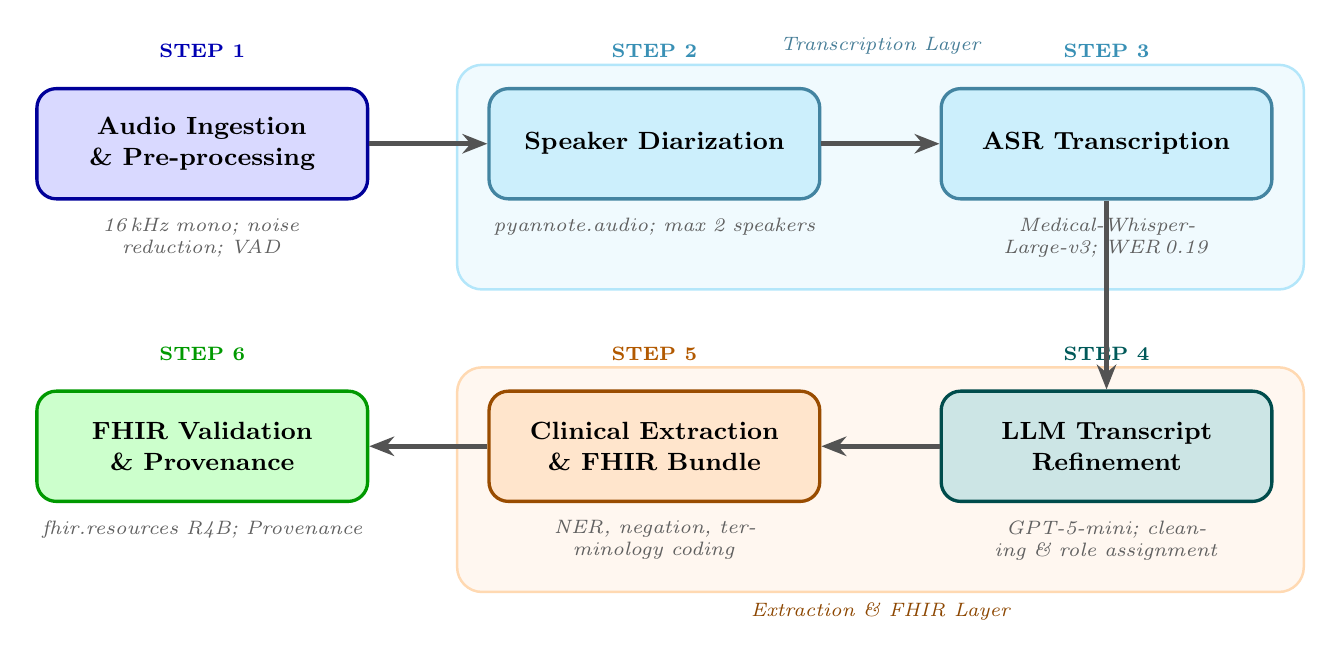
\begin{tikzpicture}[
    box/.style={
        rectangle, rounded corners=7pt,
        minimum width=4.2cm, minimum height=1.4cm,
        text centered, text width=3.9cm,
        font=\small\bfseries,
        line width=1.2pt
    },
    audio/.style ={box, fill=blue!15,   draw=blue!60!black},
    asr/.style   ={box, fill=cyan!20,   draw=cyan!60!black},
    llm/.style   ={box, fill=teal!20,   draw=teal!60!black},
    nlp/.style   ={box, fill=orange!20, draw=orange!60!black},
    fhir/.style  ={box, fill=green!20,  draw=green!60!black},
    sublabel/.style={
        font=\scriptsize\itshape,
        text=gray!75!black,
        text centered, text width=4.2cm
    },
    arr/.style={
        -{Stealth[length=9pt,width=7pt]},
        line width=1.8pt, color=gray!65!black
    },
    arrdown/.style={
        -{Stealth[length=9pt,width=7pt]},
        line width=1.8pt, color=gray!65!black,
        rounded corners=10pt
    },
]

% ROW 1
\node[audio] (step1) {Audio Ingestion \& Pre-processing};
\node[sublabel, below=0.10cm of step1] (step1-sub) {16\,kHz mono; noise reduction; VAD};

\node[asr, right=1.5cm of step1] (step2) {Speaker Diarization};
\node[sublabel, below=0.10cm of step2] (step2-sub) {pyannote.audio; max 2 speakers};

\node[asr, right=1.5cm of step2] (step3) {ASR Transcription};
\node[sublabel, below=0.10cm of step3] (step3-sub) {Medical-Whisper-Large-v3; WER\,0.19};

\node[font=\scriptsize\bfseries\color{blue!70!black},  above=0.25cm of step1] {STEP 1};
\node[font=\scriptsize\bfseries\color{cyan!70!black},  above=0.25cm of step2] {STEP 2};
\node[font=\scriptsize\bfseries\color{cyan!70!black},  above=0.25cm of step3] {STEP 3};

\draw[arr] (step1) -- (step2);
\draw[arr] (step2) -- (step3);

% ROW 2
\node[llm,  below=2.4cm of step3] (step4) {LLM Transcript Refinement};
\node[sublabel, below=0.10cm of step4] (step4-sub) {GPT-5-mini; cleaning \& role assignment};

\node[nlp, left=1.5cm of step4]   (step5) {Clinical Extraction \& FHIR Bundle};
\node[sublabel, below=0.10cm of step5] (step5-sub) {NER, negation, terminology coding};

\node[fhir, left=1.5cm of step5]  (step6) {FHIR Validation \& Provenance};
\node[sublabel, below=0.10cm of step6] (step6-sub) {fhir.resources R4B; Provenance};

\node[font=\scriptsize\bfseries\color{teal!70!black},   above=0.25cm of step4] {STEP 4};
\node[font=\scriptsize\bfseries\color{orange!70!black}, above=0.25cm of step5] {STEP 5};
\node[font=\scriptsize\bfseries\color{green!60!black},  above=0.25cm of step6] {STEP 6};

\draw[arr] (step4) -- (step5);
\draw[arr] (step5) -- (step6);

% Connecting arrow row1 -> row2
\draw[arrdown] (step3.south) -- ++(0,-0.9cm) -| (step4.north);

% Background shading
\begin{scope}[on background layer]
    \node[
        fill=cyan!6, draw=cyan!30, rounded corners=9pt, line width=0.9pt,
        fit=(step2)(step3)(step2-sub)(step3-sub),
        inner sep=8pt,
        label={[font=\scriptsize\itshape, text=cyan!55!black]above:Transcription Layer}
    ] {};

    \node[
        fill=orange!6, draw=orange!30, rounded corners=9pt, line width=0.9pt,
        fit=(step4)(step5)(step4-sub)(step5-sub),
        inner sep=8pt,
        label={[font=\scriptsize\itshape, text=orange!55!black]below:Extraction \& FHIR Layer}
    ] {};
\end{scope}

\end{tikzpicture}%
}% end resizebox

\caption{Overview of the proposed automated pipeline for mapping unstructured
clinical audio to HL7 FHIR-compliant data structures. The pipeline comprises
six sequential steps:
(1)~audio ingestion and pre-processing (16\,kHz resampling, noise reduction, voice activity detection);
(2)~speaker diarization via pyannote.audio constrained to two speakers~\cite{tran2022asr};
(3)~ASR transcription using Medical-Whisper-Large-v3~\cite{banerjee2024medasr};
(4)~LLM transcript refinement for cleaning and speaker role assignment~\cite{adedeji2024sound};
(5)~LLM clinical extraction producing a FHIR R4 Bundle via programmatic
\texttt{fhir.resources} construction~\cite{frei2025inferno};
and (6)~FHIR validation and provenance tracking~\cite{hl7fhir2022r4b}.}
\label{fig:pipeline}
\end{figure}




A central design decision is the collapse of the traditional multi-stage NLP pipeline (typically comprising SOAP segmentation, named entity recognition, negation detection, terminology normalization, and FHIR mapping as discrete components) into a single LLM extraction pass followed by schema-constrained, programmatic FHIR construction (Steps 5–6). This consolidation is motivated by Frei et al., who demonstrated a hallucination rate below 2.3\% when FHIR resources are assembled programmatically via \texttt{fhir.resources} object construction rather than generated as free-form JSON \cite{frei2025inferno}, and by Li et al., who demonstrated the feasibility of joint LLM-driven extraction and FHIR transformation \cite{li2024fhirgpt}.

All intermediate outputs are persisted to disk after each step (\path{outputs/<name>/step0N_<name>.json}). Completed steps are detected at startup and skipped, enabling iterative development and evaluation without full pipeline recomputation.

\subsection{Audio Ingestion and Pre-processing (Step 1)}

Step 1 accepts a single audio file and produces a pre-processed float32 waveform suitable for downstream ASR and diarization, using three libraries: librosa ($\geq$0.10.2) for loading, noisereduce ($\geq$3.0.0) for stationary noise suppression, and webrtcvad-wheels for voice activity detection (VAD). The mixed audio file is loaded at 16,000\,Hz and downmixed to mono via librosa. Stationary background noise is suppressed using noisereduce's spectral subtraction method, which estimates a noise profile from nominally silent regions. Voice activity is then detected using WebRTC VAD, applied over non-overlapping 20\,ms frames (320 samples at 16\,kHz) at aggressiveness level 2 on the 0--3 scale. Frames classified as voiced are retained; the remainder are discarded. The output is an \texttt{IngestionResult} containing the voiced float32 array, sample rate, total duration, \textit{speech\_ratio} (voiced frames / total frames), and source path.

Empirically, speech\_ratio $\approx 0.85$ was observed on \texttt{day1\_consultation01\_mixed.wav} (387\,s total; approximately 328\,s voiced content). Filtering silence at this stage reduces ASR transcription time and the number of non-speech segments passed to the diarization module.

\subsection{Automatic Speech Recognition (Steps 2--3)}

\subsubsection{Speaker Diarization (Step 2)}

Speaker diarization is performed using pyannote.audio 4.x \cite{tran2022asr} with the \path{pyannote/speaker-diarization-community-1} pre-trained model, executed on CPU. The pipeline is constrained to a maximum of two speakers, reflecting the doctor–patient consultation dyad. Output is a list of \texttt{Segment(start, end, speaker)} objects with generic labels \texttt{SPEAKER\_00} and \texttt{SPEAKER\_01}. Speaker role assignment (mapping generic labels to \textsc{physician} or \textsc{patient}) is deferred to Step 4, where the full transcript context is available to enable more accurate role inference. Independent evaluation on clinical dialogue has reported word-level diarization error rates (WDER) of 1.8–13.9\% under controlled conditions \cite{tran2022asr}.

\subsubsection{ASR Transcription (Step 3)}

Transcription uses \path{Na0s/Medical-Whisper-Large-v3}, a 1.55B-parameter model fine-tuned on the PriMock57 training split by Banerjee et al.\ \cite{banerjee2024medasr}. The fine-tuned model achieves a word error rate of 0.19 on the PriMock57 validation split and 0.24 on the test split, representing a 42\% relative WER improvement over the zero-shot Whisper large-v3 baseline (WER 0.33) \cite{radford2023whisper}. The model is loaded via the HuggingFace \texttt{transformers} pipeline using \texttt{torch.float32} on CPU.

For each diarized segment of duration $\geq 0.1$\,s, the corresponding audio is sliced from the waveform using integer sample indices at 16\,kHz and passed to the ASR pipeline with \texttt{language="en"}. Each transcription is emitted as a \texttt{TranscriptSegment} (fields: start, end, speaker, text) carrying the diarization label. Segments shorter than 0.1\,s are discarded to avoid transcription artefacts.

\subsection{LLM-Based Post-processing and Clinical Extraction (Steps 4--5)}

\subsubsection{Transcript Cleaning and Speaker Role Assignment (Step 4)}

Step 4 applies GPT-5-mini via the agno Agent framework with Pydantic-enforced structured output. A single LLM pass over the complete transcript performs two tasks. First, transcription cleaning: filler words are removed, medical homophones are resolved (e.g.\ \textit{ileum} vs.\ \textit{ilium}), abbreviations are expanded (e.g.\ BP $\rightarrow$ blood pressure), and drug and anatomical names are corrected to standard spellings. Second, speaker role assignment: generic labels \texttt{SPEAKER\_00}/\texttt{SPEAKER\_01} are mapped to \textsc{physician} or \textsc{patient} based on full-transcript context, exploiting clinical questioning patterns, examination language, and symptom-reporting cues. The output schema is \texttt{\_LLMTranscript}, containing a list of \texttt{\_LLMSegment} (fields: index, speaker\_role, cleaned\_text).

Combining role assignment with transcript correction in a single LLM pass avoids a redundant API call and improves accuracy through access to global dialogue context \cite{efstathiadis2024diarization, adedeji2024sound}. The original ASR text is preserved in \texttt{PostProcessedSegment\discretionary{}{}{}.original\_text} for auditability and downstream error analysis.

\subsubsection{Clinical Extraction and FHIR Resource Generation (Step 5)}

Step 5 accepts the post-processed, role-labeled transcript and uses GPT-5-mini via agno Agent with a Pydantic extraction schema, followed by programmatic FHIR construction via \texttt{fhir.resources}, to produce a validated FHIR R4 Bundle. A single LLM pass jointly performs: named entity recognition across four resource types (Condition, MedicationStatement, Observation, Procedure); negation detection (e.g.\ ``no chest pain'' $\rightarrow$ \texttt{verificationStatus=refuted}; ``possible X'' $\rightarrow$ \texttt{unconfirmed}); relation extraction to capture drug–dose, route, and frequency as structured dosage fields; implicit SOAP classification (symptoms $\rightarrow$ unconfirmed Condition; examination/laboratory findings $\rightarrow$ Observation; diagnoses $\rightarrow$ confirmed Condition; plan items $\rightarrow$ MedicationStatement/Procedure); and best-effort terminology coding using SNOMED CT for conditions and procedures, RxNorm for medications, and LOINC for observations.

The LLM output is constrained to the following Pydantic schema:
\begin{itemize}
  \item \texttt{\_Condition}: text, clinical\_status, verification\_status, snomed\_code, icd10\_code, segment\_indices
  \item \texttt{\_Medication}: drug\_name, dose, route, frequency, status, rxnorm\_code, segment\_indices
  \item \texttt{\_Observation}: text, value, unit, loinc\_code, segment\_indices
  \item \texttt{\_Procedure}: text, status, snomed\_code, segment\_indices
\end{itemize}

FHIR R4 resources are then constructed programmatically via \texttt{fhir.resources} Pydantic models rather than as free-form JSON. The bundle includes Encounter, Condition, MedicationStatement, Observation, and Procedure resources, assembled as a collection-type Bundle. The Encounter period is derived from the minimum and maximum timestamps of transcript segments. Each resource carries a custom extension encoding \texttt{segment\_indices}, linking the resource back to its source transcript segments for auditability.

This unified approach trades an accuracy ceiling (reported at 91\% semantic completeness and 0.88 interoperability for dedicated transformer-based NER pipelines with ontology-grounded normalization \cite{brens2025semantic}) for engineering simplicity and end-to-end pipeline integration. This trade-off is consistent with the demonstrated feasibility of LLM-driven FHIR transformation in the literature \cite{hong2020nlp2fhir, li2024fhirgpt}.

\subsection{FHIR Validation and Provenance Tracking (Step 6)}

Step 6 performs structural validation of the generated bundle and attaches provenance metadata to each clinical resource, using \texttt{fhir.resources} Pydantic R4B models \cite{hl7fhir2022r4b}. Validation parses each resource through its corresponding \texttt{fhir.resources} class (Condition, MedicationStatement, Observation, Procedure, Encounter, Bundle). Pydantic \texttt{ValidationError} exceptions are caught and converted to \texttt{ValidationIssue} records (fields: severity, resource\_type, resource\_id, message). The bundle is flagged \texttt{valid=True} if and only if no error-severity issues are raised; warning-severity issues are recorded but do not invalidate the bundle.

For each clinical resource, a FHIR \texttt{Provenance} resource is generated and appended to the bundle, carrying: a \texttt{target} reference to the clinical resource; a \texttt{recorded} timestamp of generation; an \texttt{agent.who} identifying the pipeline component (\path{rtm-pipeline/step05/gpt-5-mini}); an \texttt{entity.what} referencing the source audio filename; and a custom \texttt{nlp-system} extension valueString encoding the pipeline version. This approach follows the provenance extension conventions established by the SMART Text2FHIR pipeline \cite{miller2023smart}, enabling downstream consumers to reconstruct NLP provenance without rerunning the pipeline \cite{frei2025inferno}.

\subsection{Implementation Details}

The pipeline is implemented in Python 3.13, managed with uv. All inference is CPU-only: pyannote.audio and Whisper run on \texttt{device="cpu"} with \texttt{torch.float32}, with the ASR model requiring approximately 6\,GB of RAM for the 1.55B-parameter checkpoint. LLM calls are made to the OpenAI API (configured via the \texttt{OPENAI\_API\_KEY} environment variable); diarization model weights are retrieved from the HuggingFace Hub (configured via \texttt{HF\_TOKEN}). The runtime environment is NixOS, managed through devenv with direnv-based activation.






\bibliographystyle{plain}
%\bibliography{reference}

\begin{thebibliography}{99}

% --- ASR & Transcription ---

\bibitem{adedeji2024sound}
Ayo Adedeji, Sarita Joshi, and Brendan Doohan.
\newblock The sound of healthcare: Improving medical transcription {ASR}
  accuracy with large language models.
\newblock {\em arXiv preprint arXiv:2402.07658}, 2024.

\bibitem{banerjee2024medasr}
Sourav Banerjee, Ayushi Agarwal, and Promila Ghosh.
\newblock High-precision medical speech recognition through synthetic data and
  semantic correction: {United-MedASR}.
\newblock {\em arXiv preprint}, December 2024.

\bibitem{efstathiadis2024diarization}
Georgios Efstathiadis, Vijay Yadav, and Anzar Abbas.
\newblock {LLM}-based speaker diarization correction: A generalizable approach.
\newblock 2024.

\bibitem{klusty2024clinical}
Mitchell~A. Klusty, W.~Vaiden Logan, Samuel~E. Armstrong, Aaron~D. Mullen,
  Caroline~N. Leach, Ken Calvert, Jeff Talbert, and V.~K.~Cody Bumgardner.
\newblock Toward automated clinical transcriptions.
\newblock 2024.

\bibitem{papadopoulos2022primock57}
Alex {Papadopoulos Korfiatis}, Francesco Moramarco, Radmila Sarac, and
  Aleksandar Savkov.
\newblock {PriMock57}: A dataset of primary care mock consultations.
\newblock In {\em Proceedings of the Workshop on Clinical Natural Language
  Processing}, 2022.

\bibitem{radford2023whisper}
Alec Radford, Jong~Wook Kim, Tao Xu, Greg Brockman, Christine McLeavey, and
  Ilya Sutskever.
\newblock Robust speech recognition via large-scale weak supervision.
\newblock In {\em Proceedings of the 40th International Conference on Machine
  Learning ({ICML})}, 2023.

\bibitem{tran2022asr}
Brian~D. Tran, Ramya Mangu, Ming Tai-Seale, Jennifer~Elston Lafata, and
  Kai Zheng.
\newblock Automatic speech recognition performance for digital scribes: A
  performance comparison between general-purpose and specialized models tuned
  for patient-clinician conversations.
\newblock 2022.

% --- FHIR Resource Synthesis ---

\bibitem{frei2025inferno}
Johann Frei, Nils Feldhus, Lisa Raithel, Roland Roller, Alexander Meyer, and
  Frank Kramer.
\newblock Inferno: End-to-end agent-based {FHIR} resource synthesis from
  free-form clinical notes.
\newblock {\em arXiv preprint}, 2025.

\bibitem{hong2017integrating}
Na~Hong, Andrew Wen, Feichen Shen, Sunghwan Sohn, Sijia Liu, Hongfang Liu,
  and Guoqian Jiang.
\newblock Integrating structured and unstructured {EHR} data using an
  {FHIR}-based type system: A case study with medication data.
\newblock In {\em AMIA Annual Symposium Proceedings}, 2017.

\bibitem{hong2020nlp2fhir}
Na~Hong, Andrew Wen, Feichen Shen, Sunghwan Sohn, Chen Wang, Hongfang Liu,
  and Guoqian Jiang.
\newblock Developing a scalable {FHIR}-based clinical data normalization
  pipeline for standardizing and integrating unstructured and structured
  electronic health record data.
\newblock {\em Journal of the American Medical Informatics Association},
  2020.

\bibitem{li2024fhirgpt}
Yikuan Li, Hanyin Wang, Halid~Z. Yerebakan, Yoshihisa Shinagawa, and Yuan Luo.
\newblock {FHIR-GPT} enhances health interoperability with large language
  models.
\newblock {\em NEJM AI}, 1(8), August 2024.

\bibitem{miller2023smart}
Timothy~A. Miller, Andrew~J. McMurry, James Jones, Daniel Gottlieb, and
  Kenneth~D. Mandl.
\newblock The {SMART} {Text2FHIR} pipeline.
\newblock 2023.

\bibitem{riquelme2025llm}
{\'A}lvaro {Riquelme Tornel}, Pedro {Costa del Amo}, and Catalina
  {Mart{\'i}nez Costa}.
\newblock Large language models for automating structured clinical data
  standardization: {HL7 FHIR} use case.
\newblock 2025.

% --- Clinical NLP & LLMs ---

\bibitem{moldwin2021phenotyping}
Asher Moldwin, Dina Demner-Fushman, and Travis~R. Goodwin.
\newblock Empirical findings on the role of structured data, unstructured data,
  and their combination for automatic clinical phenotyping.
\newblock In {\em AMIA Annual Symposium Proceedings}, 2021.

\bibitem{brens2025semantic}
Rafael Brens, Yuqiao Meng, Luoxi Tang, and Zhaohan Xi.
\newblock Semantic {NLP} pipelines for interoperable patient digital twins from
  unstructured {EHR}s.
\newblock 2025.

\bibitem{builtjes2025leveraging}
Luc Builtjes, Joeran Bosma, Mathias Prokop, Bram {van Ginneken}, and
  Alessa Hering.
\newblock Leveraging open-source large language models for clinical information
  extraction in resource-constrained settings.
\newblock {\em Journal of the American Medical Informatics Association}, 2025.

\bibitem{saadat2025enhancing}
Saeed Saadat, Majid {Khalilizad Darounkolaei}, Mohsen Qorbani, Atefe Hemmat,
  and Sadaf Hariri.
\newblock Enhancing clinical documentation with {AI}: Reducing errors,
  improving interoperability, and supporting real-time note-taking.
\newblock {\em InfoScience Trends}, 2025.

% --- Standards ---

\bibitem{hl7fhir2022r4b}
{HL7 International}.
\newblock {HL7 FHIR} Release 4B (v4.3.0), 2022.
\newblock \url{https://hl7.org/fhir/R4B/}.

\end{thebibliography}


%USE THE BELOW OPTIONS IN CASE YOU NEED AUTHOR YEAR FORMAT.
%\bibliographystyle{abbrvnat}
%\bibliography{reference}


\end{document}
